% BatStack technical documentation
%
%
% Scott Livingston  <slivingston@caltech.edu>
% Apr-Nov 2010.


\documentclass[letterpaper]{article}

\usepackage[pdftex]{graphicx}
\usepackage{hyperref}


\title{BatStack\\ :: reference manual ::}
\author{Scott Livingston\footnote{Email by slivingston@caltech.edu}}
\date{{\small Last updated:} \today}


\begin{document}

\maketitle
\tableofcontents
\newpage
\listoffigures
\listoftables
\newpage


\section{Introduction}

The \textit{ambition} of this document is to completely describe the
operation and design of the Batlab Microphone Array Project, often
called the ``BatStack''. Note that the term ``BatStack'' refers
specifically to the individual nodes, though it may serve as a
reference to the project as a whole. This document and the project
files (firmware code, hardware designs, etc.) aspire to include a
sufficient level of detail to allow independent construction of the
entire system from nothing.  The reader is expected to have basic
knowledge of acoustics, digital electronics and core ideas from
``signals and systems.'' We strive for technical precision, rather than
scientific research motivation and exposition.  For the latter,
manuscripts are forthcoming.

\textit{Please notify me of any errors --no matter how small-- and of
  general criticism on this work.} I would in particular like to know
what is unclear or ambiguous, and which of my assumptions on the
reader's background are too strong.

Throughout the manual, we use the notation and conventions listed in
\mbox{Table \ref{notation:tbl}}.

\begin{table}[h]
\caption{Notation}
\label{notation:tbl}
\centering
\begin{tabular}{|l|l|}
\hline
\textbf{Symbol/Style}&\textbf{Meaning}\\
\hline
\hline
\texttt{monospace} & system directories, program names, sample code\\
\hline
\textit{italics}, \textbf{bold} & PAY ATTENTION! or, key terms\\
\hline
\texttt{\$} & Unix terminal, in user mode\\
\hline
\texttt{\#} & Unix terminal, in super-user (i.e., ``root'') mode\\
\hline
\texttt{>> } & Octave or Matlab prompt\\
\hline
w.r.t. & ``with respect to''\\
\hline
N.B. & ``nota bene''\\
\hline
;-P & wink, smiley face with playful tongue\\
\end{tabular}
\end{table}

Please note that, for the most part\footnote{And I will make this
  precise later.}, file naming conventions are not strict. In
particular, most (or all?) software works with the file data itself
and otherwise ignores the name chosen.  However, in some cases
(e.g. Radiance) file search filters use these name conventions to ease
your organization.


\section{Overview and motivation of system}
\label{overview:sec}

To fully understand the design (as implemented in the hardware before
you) requires some history, which I won't go into here.  It is best in
this case to consider the problem that motivates the system, and see
what minimal system features would help us achieve our scientific
goals.

To begin, we wish to study the sonar beam structure of the
echolocating bat (actually, motivated by a particular species:
\textit{E.~fuscus}, though a more widely applicable tool would be
nice).  In other words, we are interested in the spatial and spectral
characteristics of a time-varying waveform emitted from one or more
points (or ``bats'') in space.  It is acoustic, so the usual spreading
loss and atmospheric (frequency dependent) absorption issues
apply. We can address the spectro-temporal aspects of the signal by simply
recording from a microphone with appropriate filtering and
amplification to measure ultrasound. The spatial aspects of the signal
are measured by scattering the microphones throughout space, where
they act as samplers of the sound field. With proper synchronization
across channels, recordings then provide a rich view of the bat's
vocalizations: intensity and spectral information over space, which
--when traced back to the source's perspective-- reveals features of
the sonar beam structure.

More concretely from experimental data, which can readily be collected
from a free flying and foraging bat, we know that frequency content of
the signal of interest goes up to about 110~kHz.  A good target
sampling rate (given the Nyquist rate from our bandwidth) is
approximately 250~kSps\footnote{where ``kSps'' means ``1000 samples
  per second.''}.  Any ADC device has some sample width, which we
assume here to fit in 16 bits, i.e. actual sample width could be 10
bits, 12 bits, etc., but we would need 16 bits space for each
(assuming we are not packing, which could add overhead; and assuming a
byte-aligned system).

Thus, for a single channel, we would need $(16 \mathrm{~bits}) \cdot{}
(250 \mathrm{~kSps}) \approx 3.81$~Mbps\footnote{where ``Mbps'' means
  ``$2^{20}$ bits per second.''}.

Because we are interested not only in spectral and temporal
information, but also spatial, we should simultaneously measure from
many points in space.  In principle, with waveforms captured at fine
enough resolution in some region of space where a bat vocalizes, we
could characterize individual sonar beams (i.e., what the bat
generated on a particular call).  Suppose we are interested in 32
channels, i.e. sampling from 32 fixed positions in the sound field.
Then the total data throughput is $3.81 \cdot{} 32 \approx
122.07$~Mbps.  Please note that this estimate is \textit{without data
  container overhead}; that is, in practice, we would need some way to
specify which sample came from which channel, and possibly timestamps
and checksums or some other error detection/correction mechanism if we
are transferring these data far before recording them (whether on
disk, in SRAM\footnote{Static Random-Access Memory.}, etc.).

And so, our basic problem and needs are thus stated.  How do we
achieve these requirements?  What about additional design issues such
as reliability, durability, cost, ease of use, etc.?  Or features
uniquely helpful to animal behavior research?

Recording from many locations at once is not at all a new problem.
Our primary difficulty (I claim) is dealing with the high sampling
rate per channel required to record ultrasound, combined with limited
funding, or at least the desire to engineer an affordable solution to
make the resulting system generally accessible to the scientific
community.

Broadly, the array consists of two major components: an embedded
collection of local recording systems, and data management, processing
and analysis tools for a ``host computer.'' Single units of the former
are called ``BatStacks'', or simply, ``Stacks''\footnote{\textit{historical
  note:} this name is due to earlier designs by Murat Aytekin, which
had 4 or so layers of printed circuit board (PCB).}. Each Stack has a
microcontroller, 4 SRAM chips, headers for 4 microphone channels, and
some small interface-related circuitry. A microphone channel is made
up of a small electret microphone, an amplifier board, and a shielded
cable between the amplifier and its parent Stack. See Section
\ref{hardware:sec} for details on hardware design, parts, etc. See
Section \ref{firmware:sec} for a description of firmware, including
setting up a build environment (in case you wish to modify or extend
the firmware).

The host-side tools serve mainly two types of purpose: ``low level''
data manipulation and preparation, and data processing and analysis.
Some notes on ``low level'' tools are compiled in
Section~\ref{misctools:sec}. However, for such small items, comments
in the code are often the best reference, and mention of the program
in this manual is limited to in-place description as needed. Data
processing and analysis happen primarily through the application
Radiance (see Section \ref{radiance:sec}) and its visualization
companion \texttt{beamviz}.

\begin{figure}
\centering
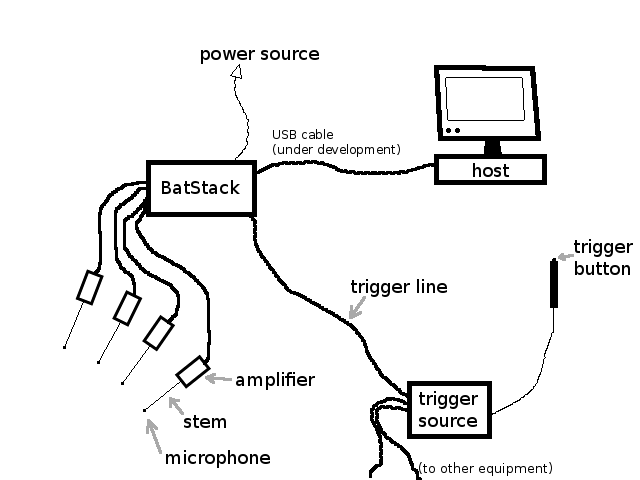
\includegraphics[width=5in]{figures/hilevel_desc.png}
\caption[High-level system description]{High-level, systems
  description of the Array. Four microphones (and attached amplifiers)
  are shown to connect to a single ``BatStack'', which receives power
  from a battery or a generic mains (i.e. wall socket power)
  supply. The BatStack is triggered externally to initiate (or stop)
  recording in synchrony with other devices.}
\label{blocksys:fig}
\end{figure}

A simplified diagram of the current deployed system (at time of
writing) is in Fig.~\ref{blocksys:fig}. After being powered on, and
given a virgin or mated SD card (cf. Section \ref{setup:sec}), a Stack
will become ready to record. The basic operation is then
\begin{enumerate}
\item Wait for trigger signal. Sample all four microphones with a
  period of 3.75 $\mu$s (hence, sampling rate is $\approx$266
  kSps). Continuously write to a cyclic buffer \textit{external} to
  the microcontroller.

While waiting, a single green LED on the Stack will flash on-and-off
slowly. This can be interpreted as a ``ready'' signal, but note that
\textit{blinking begins before a first full pre-trigger sequence of
  samples is recorded in the buffer}. That is, if you are configured
for 2 seconds pre-trigger, but then pulse the trigger 1 second after
seeing the green light begin to blink, then the first second of trial
data will be undefined\footnote{actually, either junk values or part of the
last trial.}.

\item After receiving trigger, sample and record as many post-trigger
  blocks as specified by the Stack configuration
  (cf. Section \ref{config:sec}). E.g., I typically use an end-trigger, where
  the last (approximate) 4 seconds up to the trigger itself are
  recorded.

Upon triggering, the ``ready'' light stops periodic blinking and will
not recommence until Stack is ready for the next trial.

\item Then dump the captured trial to an attached SD card (or some
  other bulk storage; other possibilities are under consideration). For
  a full (approx. 4 seconds) recording, copy time is about 1 minute.

To indicate activity, a green LED on the Stack toggles for each block
transferred to the SD card. Most likely this light will blink so
quickly that you will not notice it (i.e., it will appear continuously
on) but occasionally block writes are delayed, which will be visible
by prolonged moments of light on or off.

\item Assuming no fatal errors are encountered, prepare for and return
  to ``ready'' state, thus waiting for the trigger signal of the next
  trial.
\end{enumerate}

Stacks may be powered off whenever they are ready to be
triggered. Hard kills at other times could corrupt the contents of
bulk storage (i.e. the SD card).

After an experiment session completes, the investigator
\begin{enumerate}
\item gathers all SD cards (one per Stack);

\item saves results to a host machine by running
  \texttt{dumpsd}\footnote{\texttt{dumpsd} is under
    ``src/util/dumpsd'' in the BatStack source tree.} (cf. Section
  \ref{usage:sec}) on each card in succession; and

\item for each trial, combines data from separate stacks into single
  array data files (See Section \ref{array_format:sec} for
  specification)\footnote{This step requires knowledge of your chosen
    global numbering scheme, i.e. which microphone is channel 1, which
    is channel 2, and so on. Accurate labels are critically important
    for calibration, data management and analysis.}.
\end{enumerate}
Given calibration (cf. Section \ref{setup:sec}) measurements, the
investigator can then begin marking vocalizations in Radiance
(cf. Section \label{radiance:sec}) and start scientific analysis. As
stated earlier, processing and analysis of microphone array data are
distinct from recording. That is, once trial data files are generated,
any tool may be used (or newly developed) that recognizes the file
specification (cf. Sec. \ref{array_format:sec})\ldots your methodology
is not restricted to the Radiance or \texttt{beamviz}
applications\footnote{Indeed, one of my design goals is modularity.}.

\section{Usage, or How to be a ``badass''}
\label{usage:sec}

In this section, we will step through all major aspects of usage:
construction, installation, testing, calibration, experimental
recordings, and data manipulation. This is written in tutorial fashion
with plentiful footnotes and links to other more detailed and
referential parts of the manual where appropriate. Unlike other
sections, you should treat this part as a story, told by a
campfire. So grab a neighborly cup of coffee, and let's begin.

\subsection{Construction}
\label{construct:sec}

As noted in Section \ref{overview:sec}, the Array consists of two
major divisions: a localized recording system\footnote{``localized''
  in the sense that there are many small nodes at which the magic
  happens and distributed in your experimental setup (e.g. within a
  flightroom or anechoic chamber).} and a collection of
host-computer-based\footnote{``host-based'' or ``host computer''
  refers to stuff meant for your use on a ``typical'' or ``personal
  computer'', e.g. Octave/Matlab scripts.} tools for data processing,
manipulation and analysis. Only the former requires hardware
construction, if you do not have a pre-built rig.

An implemented Array (i.e., any particular physical installation) is
made up of groups of 4 microphones\footnote{or rather, up to 4
  channels per node; unused channels are left floating; or better,
  grounded.} Each group is orchestrated, at its heart, by a pair of
small electronics boards, which we refer to here loosely as a BatStack
or \textit{Stack}. The Stack consists of an \textbf{MCU
  board}\footnote{MicroController Unit.}, \textbf{memory
  board}\footnote{also called ``SRAM board'' because it uses Static
  Random-Access Memory (in the current design).}, SD card holder,
trigger interface, and channel header mini-board. The last three items
exist exclusively as patchwork to older designs. New MCU and memory
boards incorporating these and other improvements are under
development.  Each one of the four possible channels for a Stack uses
an amplifier with attached microphone and a shielded cable for
providing the amplifier with power and for receiving its analog
measurements.

Before considering specific components, here is some general advice
(similar in purpose to stuff in Section \ref{tips:sec}). These are my
opinion and, at times, intentionally unnecessarily polemic.
\begin{itemize}
\item {\large \textbf{\textit{Wear safety glasses}}, at least, and
  follow other precautions and safety guidelines as appropriate.} I do
  not care how experienced you are. This is a demand, not a suggestion.

Relatedly, after working with electronics stuff, you should wash your
hands before eating, drinking or kissing.

\item You should assemble electronics in the order of increasing
  delicacy. When populating\footnote{i.e., ``putting electrical parts
    on,'' thus helping a PCB achieve its \textit{raison d'\^etre}.}
  PCB, first make any mechanical changes necessary, such as smoothing
  corners or breaking a repeated print into individual pieces, if left
  uncut from the factory. Second, solder all passive parts, beginning
  with the most heat-tolerant and low-cost items\footnote{Resistors
    and capacitors of standard values (e.g. 1 k$\Omega$, $\frac{1}{4}$
    W, 1\% tolerance) are very cheap.}. Finally, solder
  ICs\footnote{integrated circuit.} in whatever order reduces heat
  exposure greatest, with preference given to those most sensitive.

My suggested order \textit{should be changed} depending on particular
structural constraints. For example, attaching a cable header (which
is very heat tolerant) before a small surface-mount IC (which is more
delicate) may make soldering the latter impossible. The take-home
message: \textit{plan ahead}. Understand the whole assembly process
before beginning any specific part.

\item Debugging later can be hell, so make note of potential weak
  points during an assembly job. These provide quick checkpoints while
  looking for problem sources later during testing. Be aware that
  damaging parts is often not a binary process; that is, a burnt op
  amp chip may show poor or decaying response over time in the field,
  despite initial decent performance.

\item The most expensive single parts of the Array hardware are the
  microphones and the SRAM chips (or rather, the combined market value
  of a populated memory board --4 to 8 SRAM chips-- is high). Keep
  this in mind during construction.

\item Include your precious time in cost considerations. Do not be
  afraid to simply throw away failed electronics, or rather, place
  them in the junk/spare parts box. Similarly, buying high quality
  equipment may be better than spending weeks hacking on mediocre
  tools from the 1970s.

\item If you are soldering several rows of male header pins (0.1"
  spacing; generic), then I highly suggest you place them into
  something that matches the size of their target female
  socket\footnote{This can be the target electronics, but be sure the
    latter can tolerate repeated exposure to soldering iron
    heat!}. Doing this is a good practice to be confident the
  completed parts will all fit together. Reflowing the solder later is
  unpleasant and may damage nearby components if the excessiv heat is
  not managed well.
\end{itemize}

We begin by describing construction of the microphone amplifier, in
the sequel, followed by MCU and memory boards (with SD card holder and
channel header) and concluding with the trigger input.

\subsubsection{Microphone amplifier}

A parts list\footnote{known in the trade as a ``bill of materials.''}
is provided in Table \ref{mic_parts:tbl} (in Section
\ref{hardware:sec}). Note that the listed package
types\footnote{sometimes called ``footprint.''} are for the current
board design, called ``r2'' for ``release 2.'' It is still undergoing
some testing, but initial results are all good. Since the current
boards have not yet been deployed, most construction and installation
discussion concerns the previous design. To order parts for the
previous (old) boards, buy the \textit{through-hole} counterparts to
all passive components\footnote{i.e., resistors and capacitors.}.

The purpose of the ``amplifier'' is to filter the signal coming from
the attached electret microphone\footnote{Electret microphones are
  essentially capacitors with a permanent charge distribution, such
  that movement in the plates causes changes in voltage across the
  plates.}. We currently expect Knowles FG-3629 microphones.

\begin{figure}
\centering
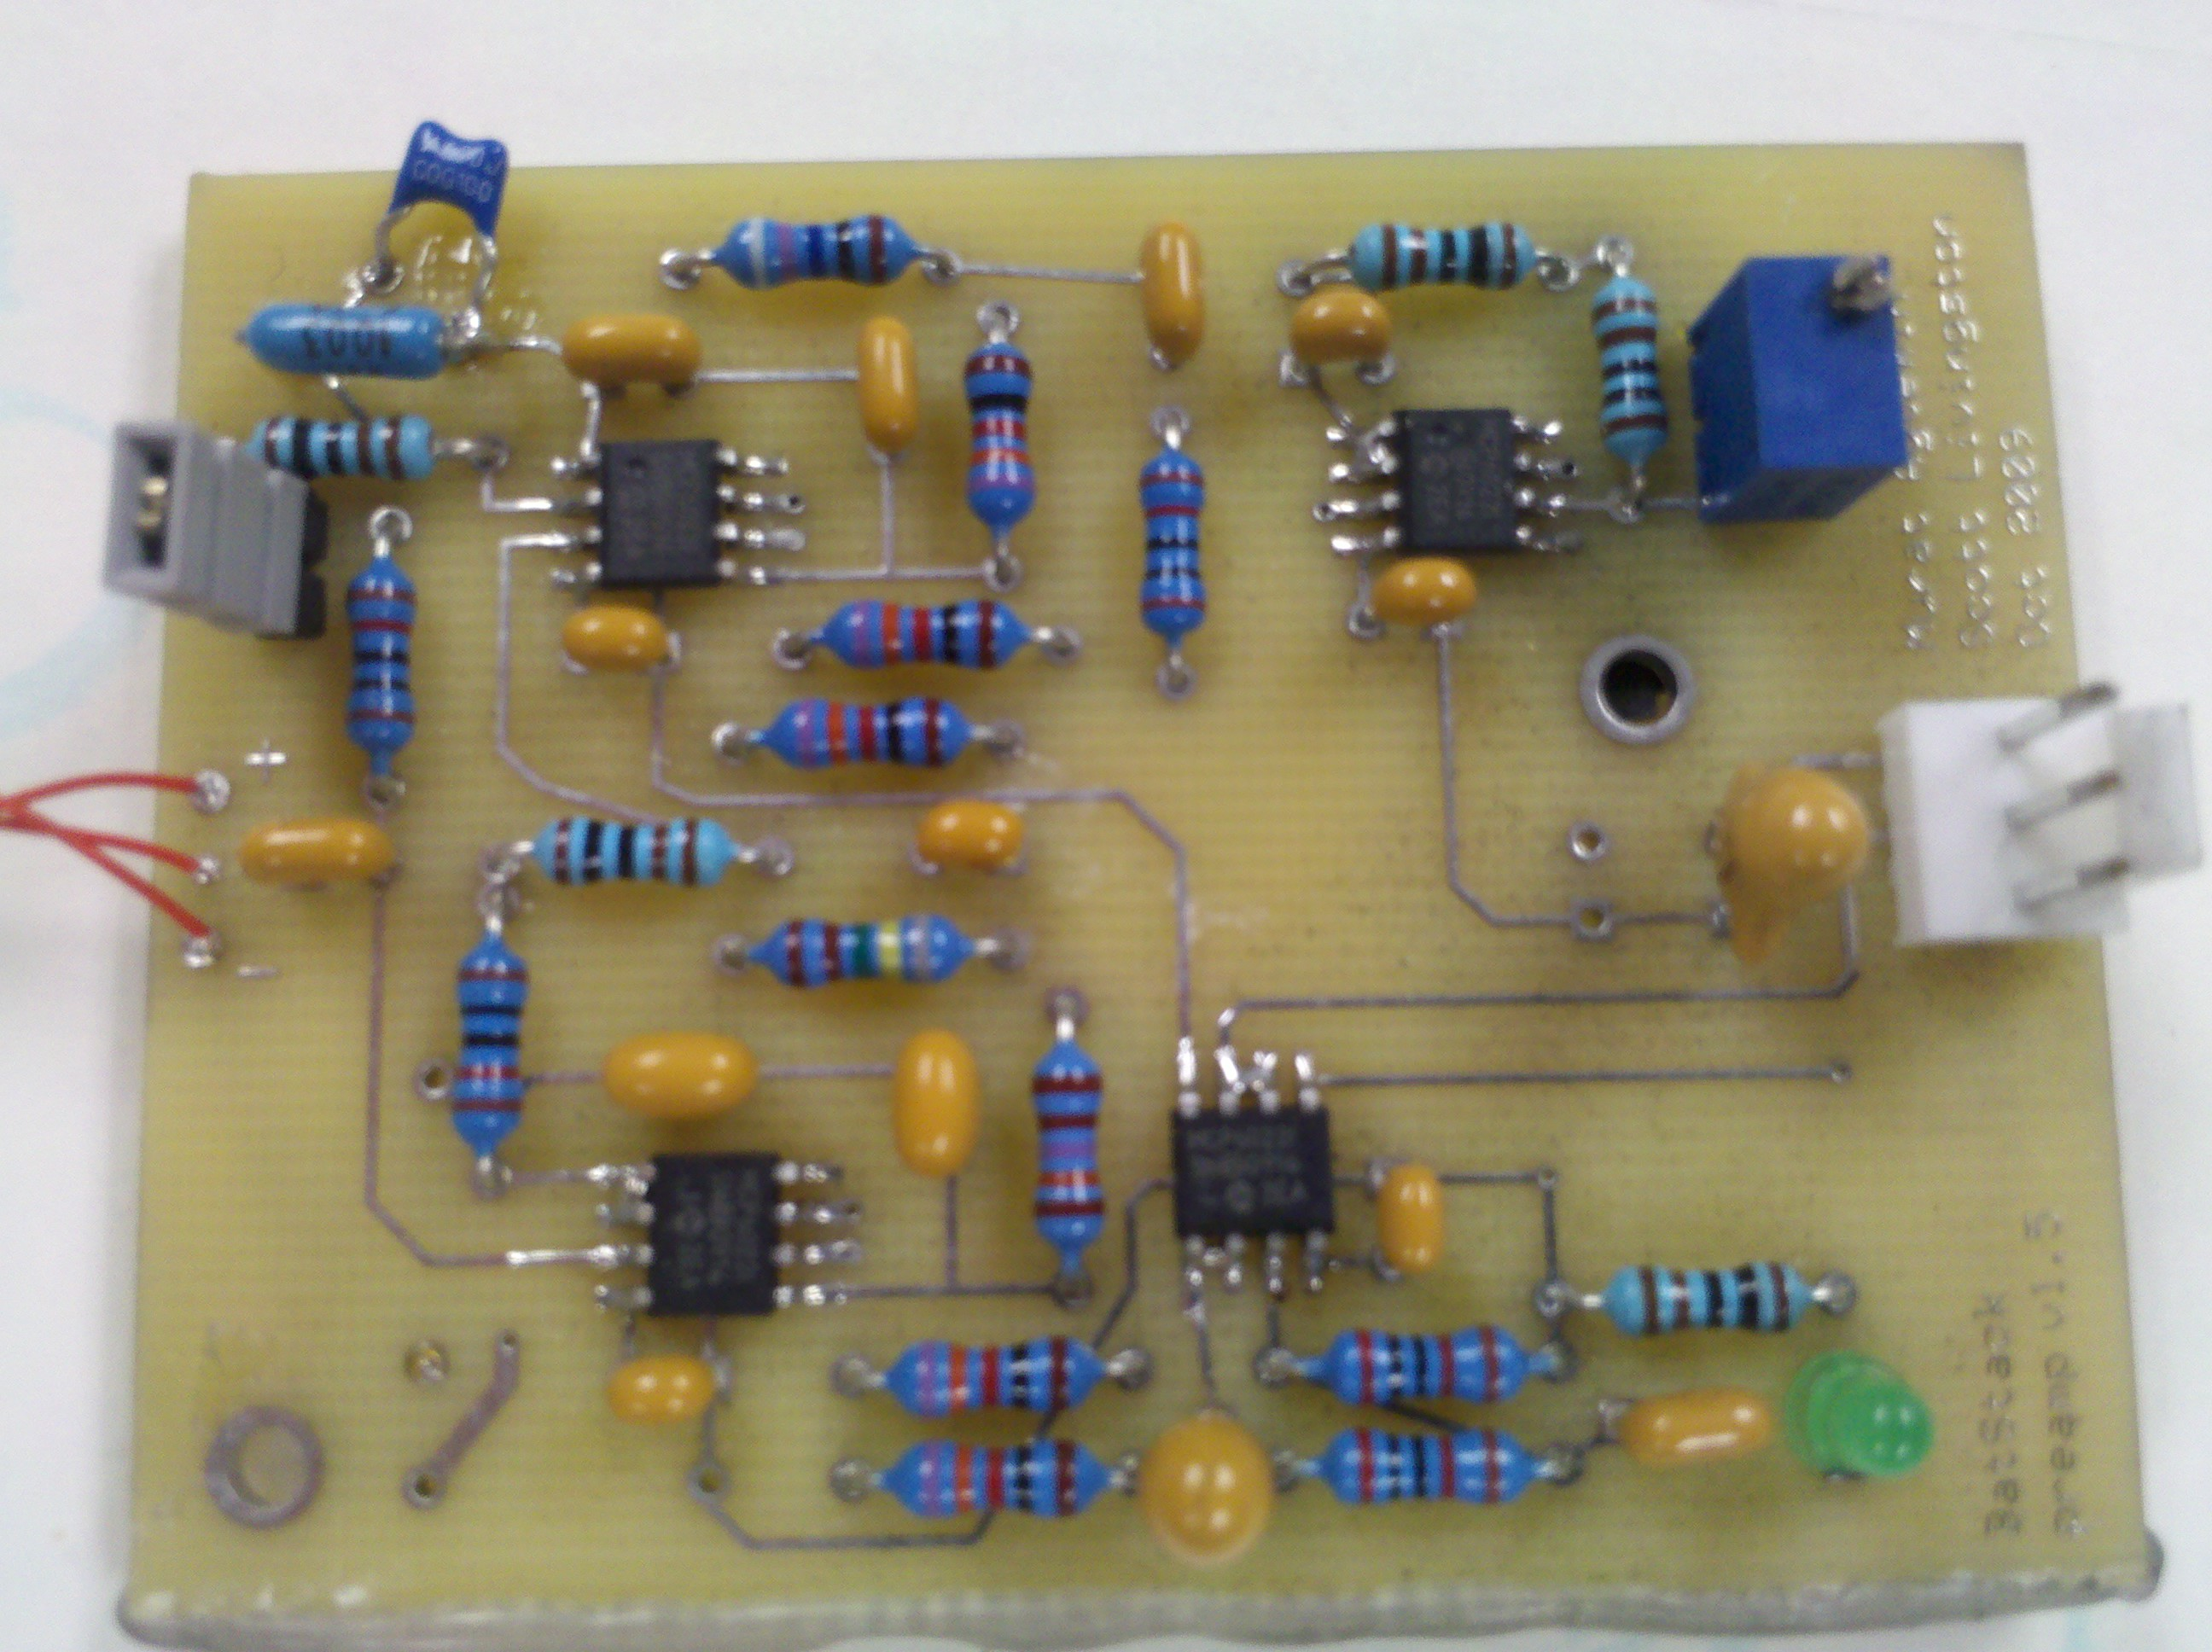
\includegraphics[width=5in]{figures/old_preamp_board.jpg}
\caption[Previous (old) microphone amplifier]{Previous (old)
  microphone amplifier. The microphone attaches to the left end of the
  board, and the power/signal cable to the right (at the white 3-pin
  header). If you look closely at the board where the microphone wires
  connect, there is a ``--'' to indicate ground, and a ``+'' to
  indicate the positive voltage supply. The middle wire carries the
  acoustic signal. Similarly, with respect to the orientation in the
  present photograph, the three pins on the cable header from top to
  bottom are external power supply (3.3V), signal and ground. Gain can
  be adjusted by turning the knob on the blue trimpot in the upper
  right corner of the photograph. See main text for additional
  details.}
\label{oldpreamp:fig}
\end{figure}

\begin{figure}
\centering
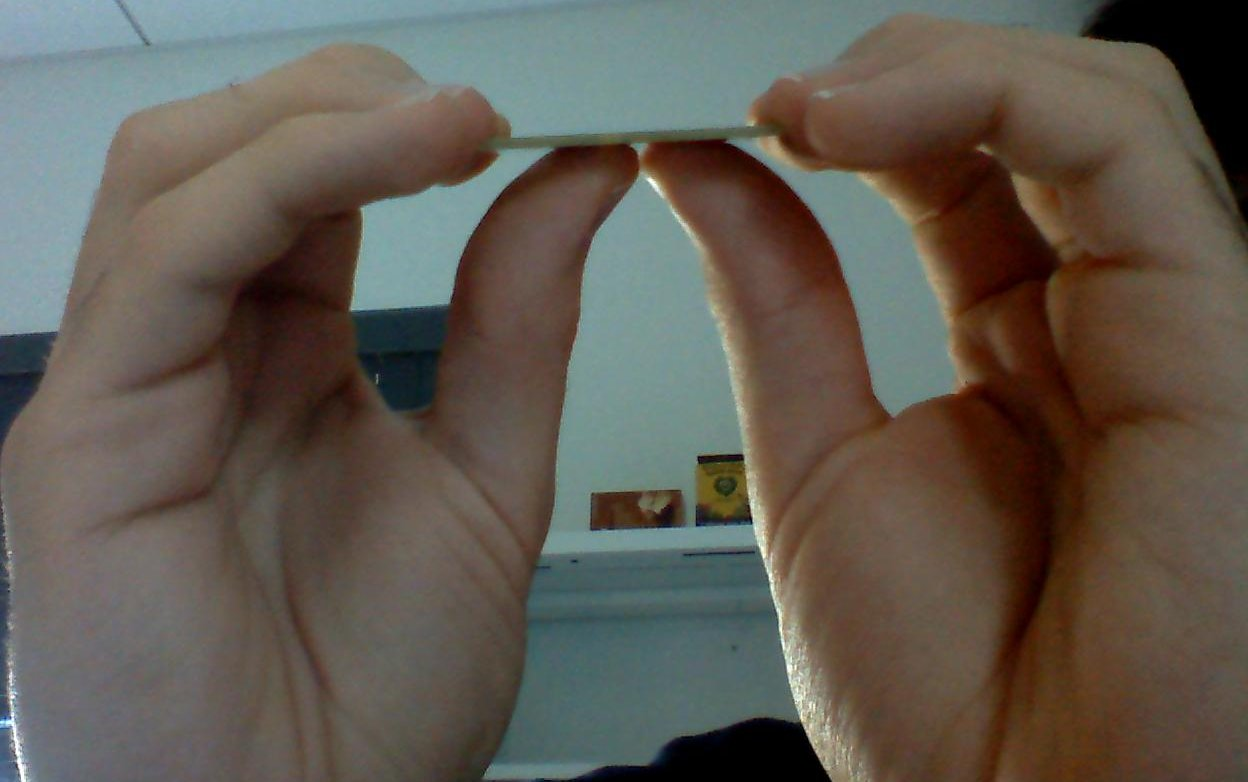
\includegraphics[width=4in]{figures/oldmicamp_board_break.jpg}
\caption[How to break virgin amplifier boards]{Example hand position
  for breaking a virgin amplifiers board (which has two copies of the
  amplifier circuit) into two pieces.}
\label{oldpreamp_break:fig}
\end{figure}

To construct a new amplifier board, use an existing, built board as a
reference and match components. An example is shown in
Fig.~\ref{oldpreamp:fig}. A circuit schematic is presented in Figure
\ref{micamp_schem:fig}. The current board requires several special
considerations.
\begin{itemize}
\item To save on costs, amplifier circuit boards were shipped as
  pairs. That is, a virgin board actually contains two amplifier
  circuits\footnote{This should be obvious from brief examination of a
    board.}. To facilitate separation (again, given limitations of
  low-cost), there is a straight mid-line of vias along which the
  board should be broken into two pieces (hence two amplifiers). 

This can be achieved by the following steps. Cutting and breaking here
will cause metal and
FR-4\footnote{\url{http://en.wikipedia.org/wiki/FR-4}} debris to
fall. Please wear protective glasses and clean up after yourself.
\begin{enumerate}
\item With the inner sharp edge of pliers or with general-purpose
  workshop-grade cutters, make a small cut from each edge along this
  mid-line. \textit{Aim to stay along the via hole centers.}

\item Hold board with fingers mounted on board edges parallel to the
  midline (i.e., the line of vias along which the board will be
  broken), and press your thumbs on the midline, as suggested in
  Fig.~\ref{oldpreamp_break:fig}.

\item Push your thumbs forward while curling your fingers back. The
  board will begin to break (listen for faint splitting sounds; FR-4
  is largely fiberglass, and yields sounds like what you might
  expect). Once some progress has been made, flip the board over and
  repeat from the other side. The idea is thus to break along the
  midline without damaging the nearby circuit.

\item Once the two pieces are separated, use pliers to pull out
  remaining metal vias (that had demarcated the mid-line). Smooth the
  now bumpy edge with a file to eliminate any sharp points (this
  doesn't require much filing, if any; the goal is only to erase
  dangerous, jagged protrusions; smooth bumps are OK).

\item Use a hot glue gun\footnote{you know, the kind from primary
  school ``arts \& crafts'' class. It is non-toxic, easy to use, and
  hours of fun.} to seal the edges along which you separated the
  amplifier boards, which you now have two of. The goal is to provide
  final assurance that the broken edge is cleanly covered and ready
  for application in the field, without fear of FR-4 bits, etc.

\item On the bottom edge of the example board in
  Fig.~\ref{oldpreamp:fig}, the results of the described splitting
  process can be seen. The non-linear translucent material along the
  edge is dried ``hot glue'', and the semi-yellow grating apparent
  beneath it are the stripped via holes.
\end{enumerate}

\item The original circuit, for which the PCBs you are using were
  designed, included two trimpots\footnote{a type of variable
    resistor; probably in a small blue rectangular case with a metal
    adjustment knob. Use small flathead screwdriver to adjust. You can
    tell an extremum has been reached by listening for a faint
    click.}: one near the microphone attachment point (upper-left of
  Fig.~\ref{oldpreamp:fig}) and the other near the power/signal cable
  header (upper-right of Fig.~\ref{oldpreamp:fig}). The trimpot near
  the microphone has since been replaced with a fixed 100~k$\Omega$
  ($\leq$1\% tolerance, etc.)  resistor. As usual, a potentiometer has
  three leads, and here we short two of them. Thus, when fitting the
  100 k$\Omega$ resistor into the trimpot's location, be aware that
  only two (out of three) positions are possible.

\item Both high gain feedback paths require low Farad bypass
  capacitors. If you are looking down at the board such that the
  power/signal cable header is toward your right side and the
  microphone is toward your left (as in Fig.~\ref{oldpreamp:fig}),
  then the two high gain steps are in the
\begin{enumerate}
\item upper right, where the 100~k$\Omega$ trimpot sits, and

\item upper left, where the 100~k$\Omega$ permanent resistor was placed
  (see previous item).
\end{enumerate}
  In the assembled amplifier boards that you are (hopefully) using for
  reference, I placed a 68~pF ceramic capacitor in parallel with these
  resistors. The former requires attachment on the board's underside;
  I covered the protruding result with black electrical tape to
  prevent shorts\footnote{\textit{Jargon:} a ``short'' is a very low
    Ohm (i.e. low resistance, e.g. a wire) connection between two
    nodes, typically assumed to be unintentional.}. The latter can be
  soldered in parallel on the topside; you can see the small blue
  capacitor near the far corner of the board, as in the Figure.

\item Many of the assembled amplifiers have a jumper on the
  microphone-end of the board, as on the left in the example shown in
  Fig.~\ref{oldpreamp:fig} (hint: the jumper is gray). This was added
  originally to facilitate experimenting with different offset
  voltages\footnote{This is a single-supply design; hence, our signal
    of interest rides on a DC offset voltage --sometimes called the
    ``virtual ground''-- midway between the power rails.}. While
  constructing new boards, you can safely make this jump permanently
  connected with a \textbf{short} piece of \textbf{thick} wire.

\item In assembled boards you will see some unused pin holes. In
  particular, these are
\begin{itemize}
\item two large holes for mounting the amplifier in your experimental
  setup, that are not a part of the circuit;

\item an extra pair of component holes near the power/signal cable
  header, which allow a second tank capacitor to be placed in parallel
  with the present one (cf. mid-right of photo in
  Fig.~\ref{oldpreamp:fig}); and

\item two unused resistor positions near the microphone (lower-left of
  Fig.~\ref{oldpreamp:fig})\footnote{These are to facilitate
    experimenting with different power supply values, which informal
    tests for 5~V suggest not to improve SNR (signal-noise
    ratio).}. See Sec. \ref{hardware:sec} for details.
\end{itemize}
\end{itemize}

\subsubsection{MCU and memory boards}

In the current release, there are three PC boards\footnote{Printed
  Circuit Board, PCB.} and two custom components that make up a single
Stack. These are
\begin{enumerate}
\item MCU board (cf. Fig.~\ref{oldmcu:fig}),

\item memory board (cf. Fig.~\ref{oldmem:fig}),

\item headers for amplifier power/signal cables (not depicted in a figure),

\item SD card holder (also not depicted in a figure), and

\item trigger input.
\end{enumerate}

\begin{figure}
\centering
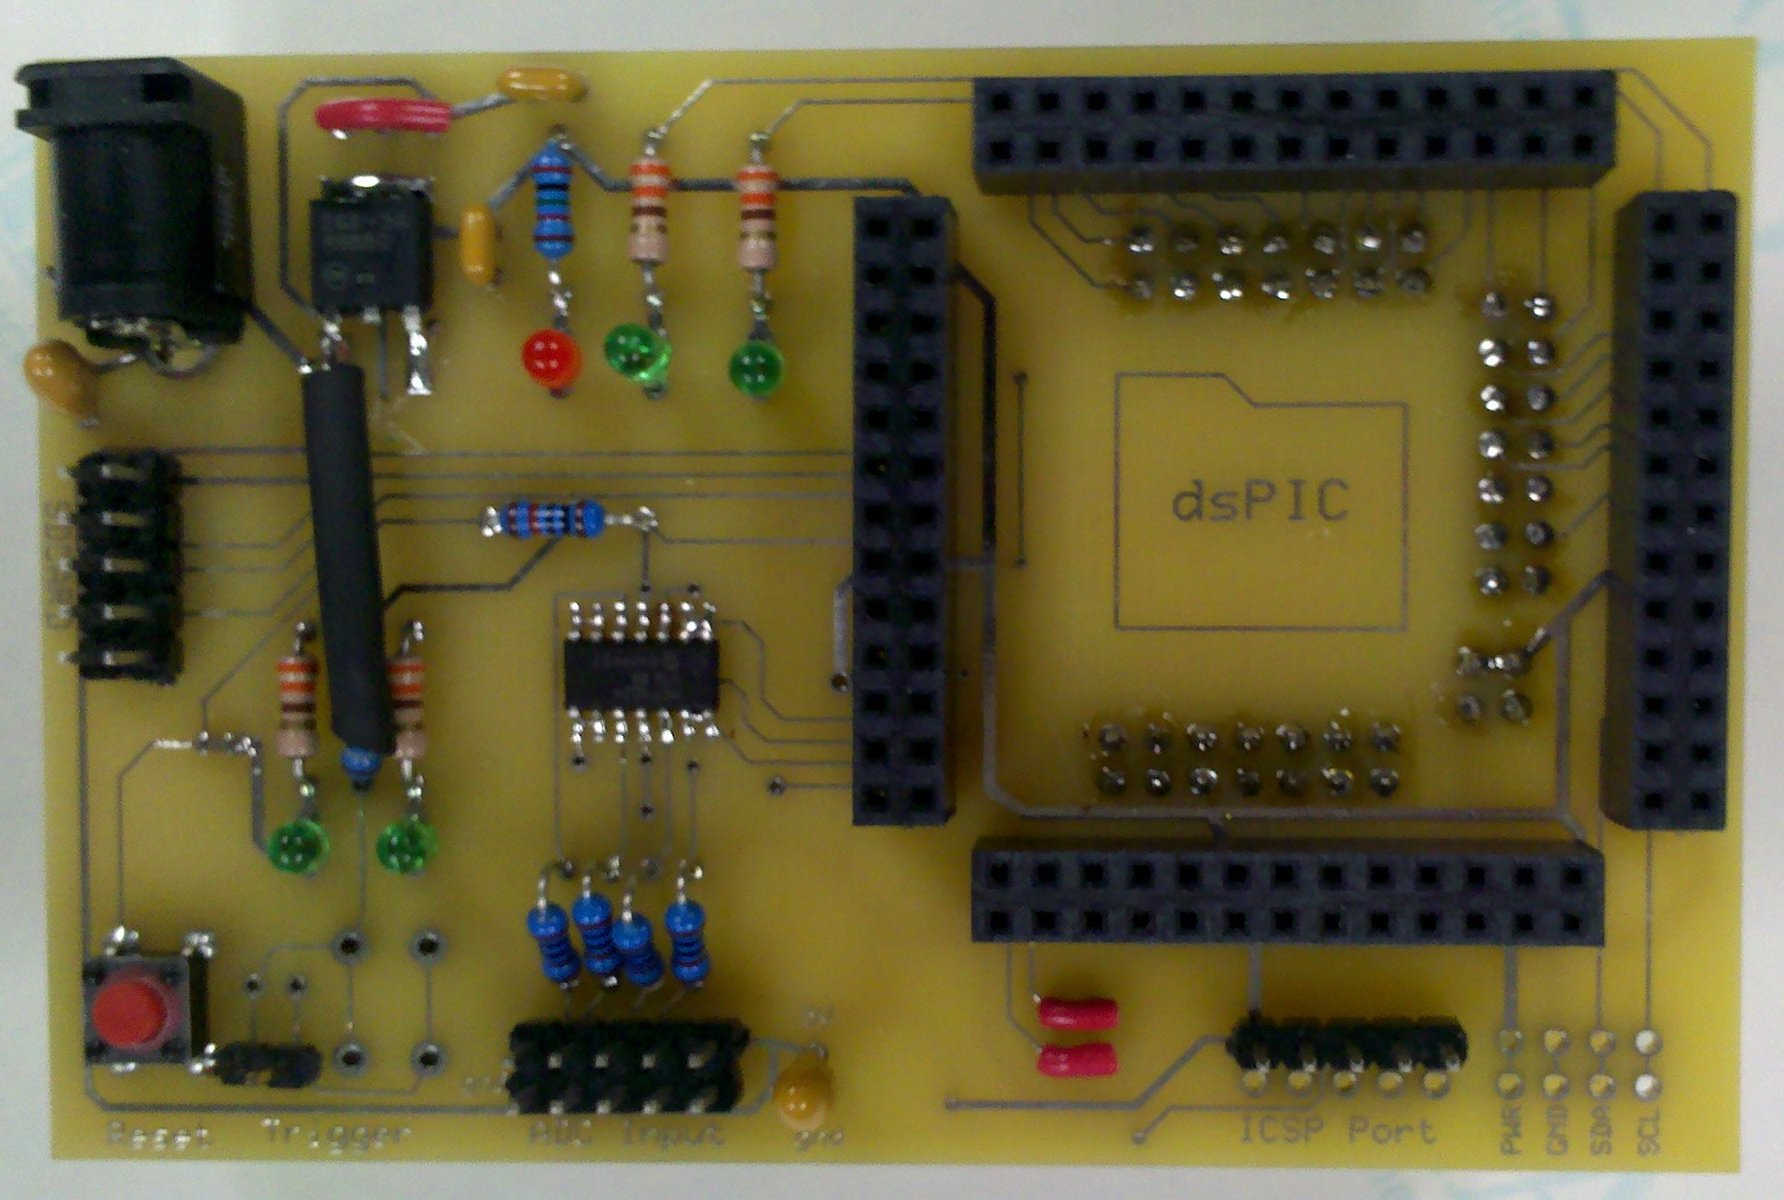
\includegraphics[width=\textwidth]{figures/old_mcu_board.jpg}
\caption[Current microcontroller board]{Current MCU board. Grossly,
  the dsPIC33F chip breakout (cf. Fig.~\ref{mikropic:fig}) attaches on
  top on the right, and the memory board (cf. Fig.~\ref{oldmem:fig})
  attaches underneath. Power supply is provided via the black jack in
  the upper-left corner. Various patches are visible (e.g., scratched
  off trace and heat-shrink-covered jumper in mid-left region). Note
  that \textit{this is a complete, populated board}; i.e., exposed
  holes are for uncessary parts. See main text for details.}
\label{oldmcu:fig}
\end{figure}

\begin{figure}
\centering
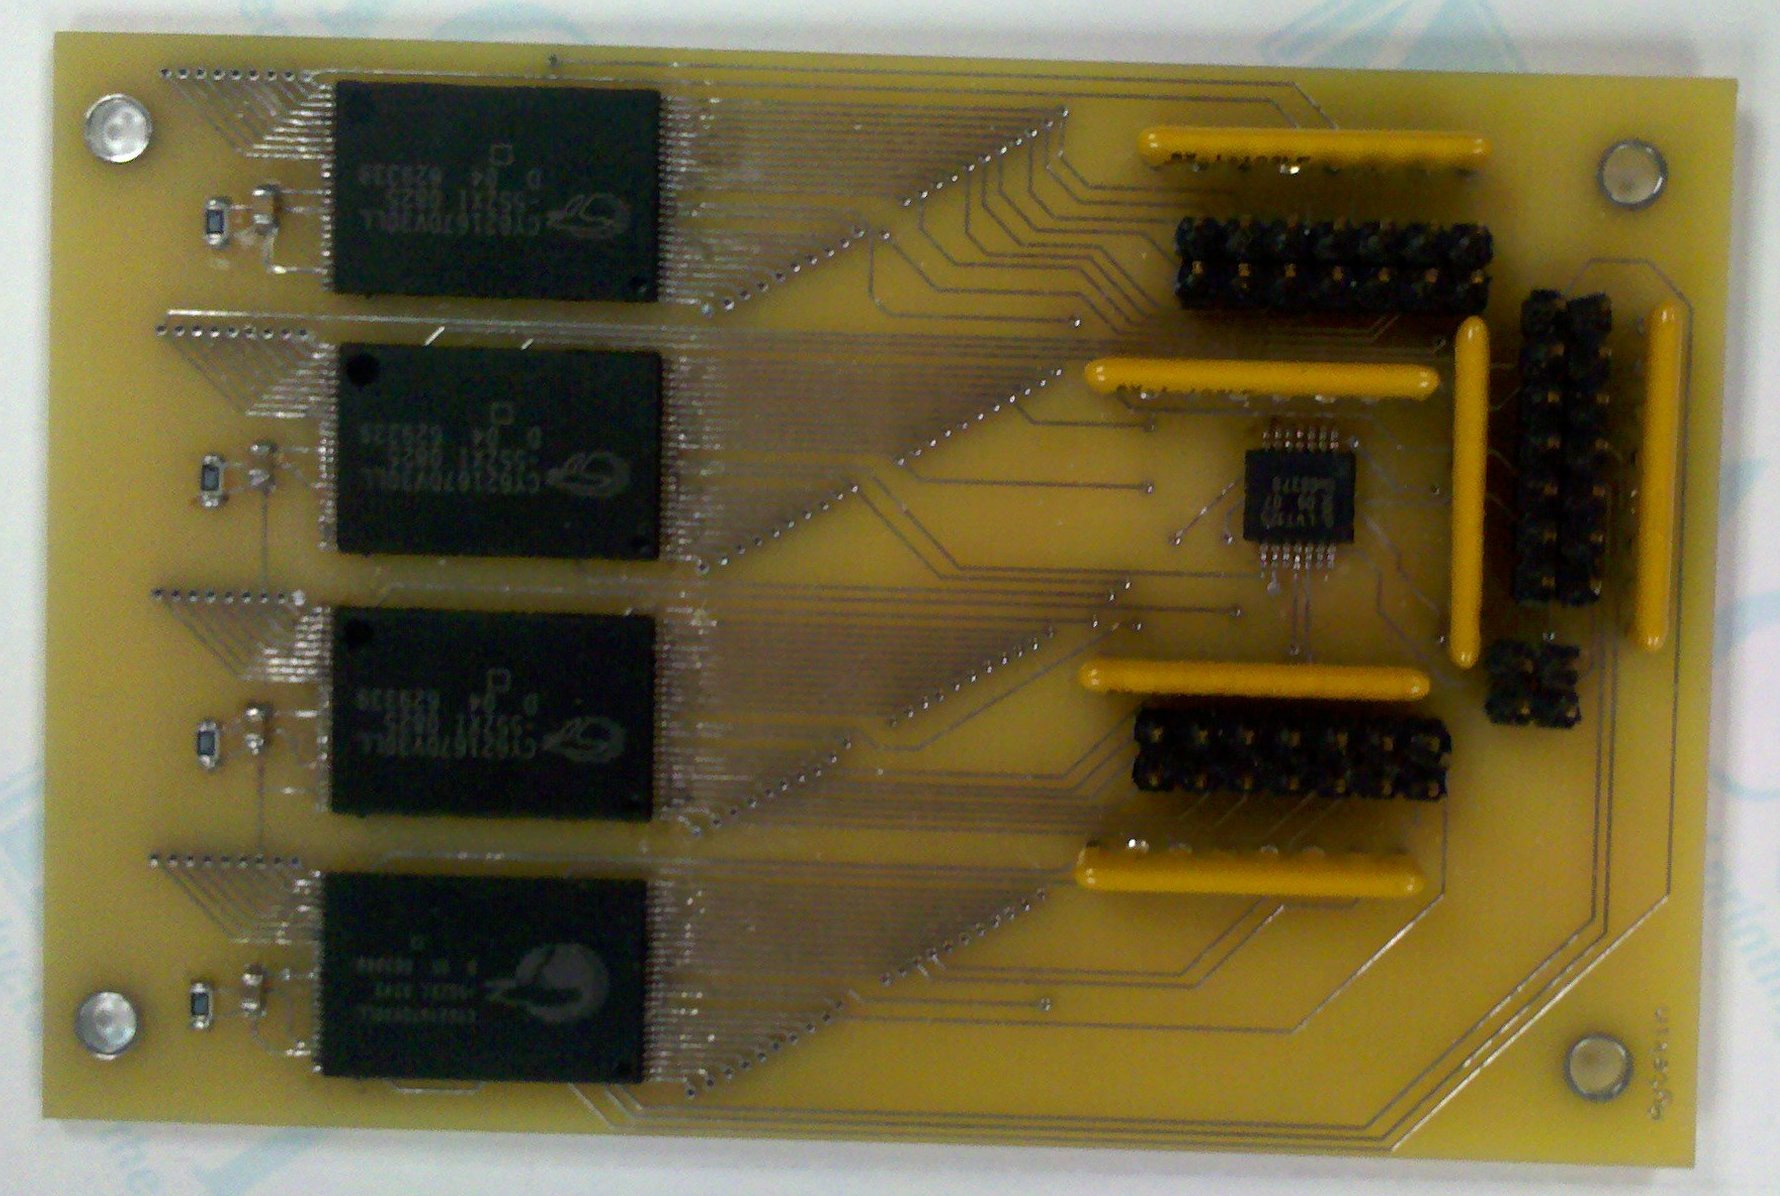
\includegraphics[width=\textwidth]{figures/old_mem_board.jpg}
\caption[Current memory board]{Current memory (or ``SRAM'')
  board. Four SRAM chips can be seen on the left; buffer chip and
  mount point on the right. See main text for details.}
\label{oldmem:fig}
\end{figure}

\begin{figure}
\centering
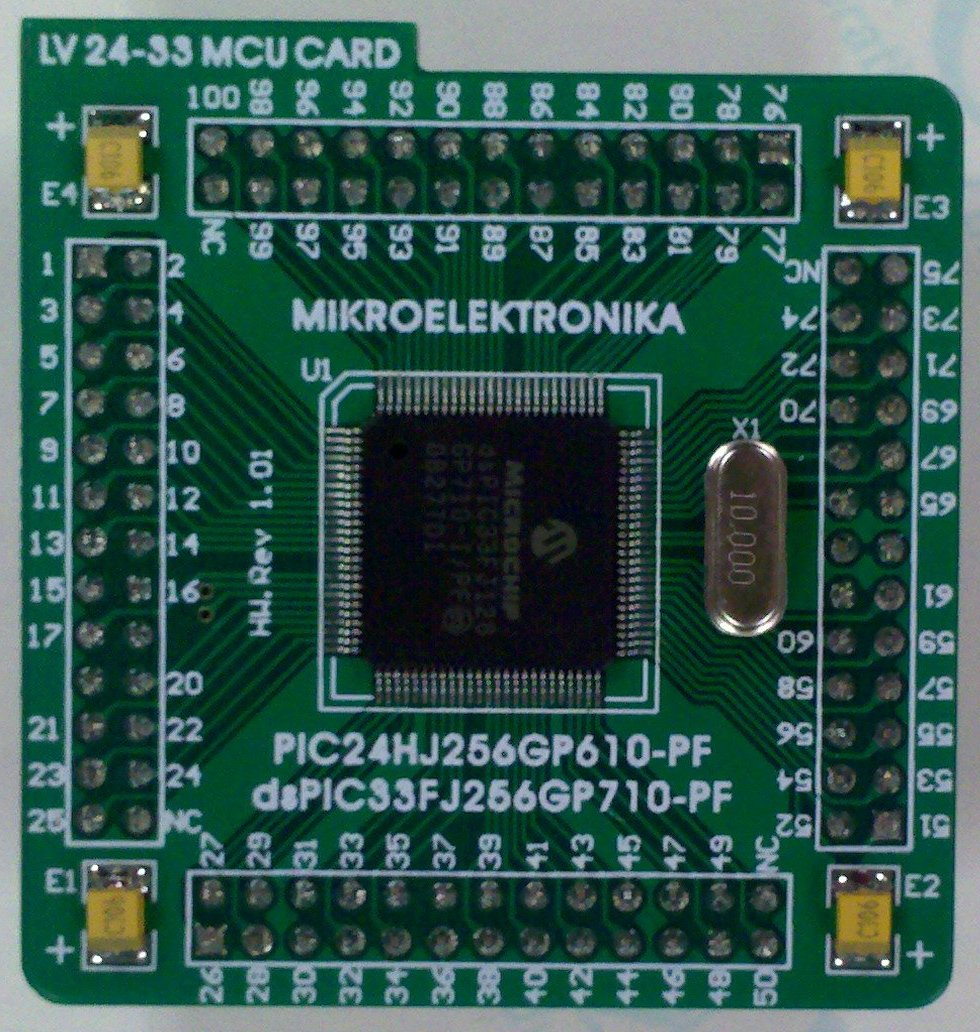
\includegraphics[width=2.5in]{figures/mikro_dspic_breakout.jpg}
\caption[MikroElektronika dsPIC33F breakout LV 24-33 board]{LV 24-33
  dsPIC33FJ128GP710 (100-TQFP) breakout, includes 10~MHz crystal;
  mfg. by MikroElektronika (company website:
  \url{http://www.mikroe.com}).}
\label{mikropic:fig}
\end{figure}

Once again, constructing the MCU and memory boards is largely a
cloning job: simply make new boards that are functionally identical
(within component manufacturing tolerances) to existing, populated
boards. A circuit schematic is presented in Figure
\ref{mcubrd_schem:fig} (you will need to ``zoom in'' to view
detail). An example complete MCU board --sans dsPIC33F chip
breakout\footnote{\textit{Jargon:} a ``breakout board'' essentially
  provides access to pins in a manner different from that available on
  the manufactured package; usually to ``break out'' means to make
  more easily accessible for development and debugging, though with
  corresponding costs incurred for space usage, introduction of
  various noise types, etc. However, a breakout board may provide
  additional components, such as that of the dsPIC33F shown in
  Fig.~\ref{mikropic:fig}.}-- is shown in Fig.~\ref{oldmcu:fig}; the
prominent socket holds the dsPIC33FJ128GP710 chip breakout, shown in
Fig.~\ref{mikropic:fig}. An example complete memory board is given in
Fig.~\ref{oldmem:fig}.

Admittedly, the existing, built MCU boards vary some in their
appearance. The one in Fig.~\ref{oldmcu:fig} looks to be missing some
parts, and includes several jumped wires (e.g., along the top left,
near the $3.3$V voltage regulator). This is due to evolution of the
design, and related hardware patches. Until a new design
ships\footnote{Scott is still working on these; please contact about
  collaboration if interested.}, you will need to apply these patches
manually\footnote{small changes can be applied to the current MCU
  board layout to effectively induce these patches permanently. This
  is appropriate if you need expediency; look in the BatStack
  sourcetree under \texttt{hardware/archived} for corresponding
  ExpressPCB (\url{http://expresspcb.com/}) layout files. See Section
  \ref{hardware:sec} for details.}.

We mention here the patches and other noteworthy items for
construction of the MCU board. All references to ``the Figure'' are
for Fig.~\ref{oldmcu:fig}, and ``the example board'' (or simply, ``the
board'') is regarding what is shown in Fig.~\ref{oldmcu:fig}. For more
general design discussion, see Section~\ref{oldmcu:sec}. If some trace
pathways are confusing, looking at the old and slightly different
layout in Fig.~\ref{oldmcu_layout:fig} may be helpful because top and
bottom layers are simultaneously visible.
\begin{itemize}
\item The example board is \textit{minimally populated}, in that only
  crucial components --aside from the red LED (power indicator),
  which is helpful but not necessary-- are present.

\item Despite the labeling, the ICSP\footnote{In-Circuit System
  Programming.} port (in the lower right region of board) is in a
  non-standard configuration. Confer Sec.~\ref{oldmcu:sec}.

\item The red-insulated jumper wire near the power supply is necessary
  because a 5~V voltage regulator previously provided a bridge between
  the external supply and the 3.3~V regulator (in addition to
  supplying 5~V for some parts of the Stack that needed it); the 5~V
  regulator has since been removed from the design, so we bridge the
  gap with a jumper wire, thus providing the external supply directly
  to the 3.3~V regulator.

\item Becoming visible from the middle-lower edge of the 3.3V
  regulator chip, there is a trace which must be broken,
  i.e. physically scratched off to break the electrical
  connection. This is apparent in the Figure, where my scratch marks
  can be seen as slightly more-white-than-yellow, relatively to nearby
  PCB. This is important and \textit{must be done before providing
    power to the assembled board}. Otherwise, parts may burn.

\item \textbf{The following only applies to some MCU boards.} We
  expect to trigger on a rising edge --or more accurately, a pulse
  from a baseline of 0~V-- and hence, the corresponding pin of the
  dsPIC33F chip should be pulled down. Recent MCU
  boards\footnote{there should not be many remaining, as I recall.}
  are designed for the converse, i.e. trigger on pulse to 0 from
  baseline of 3.3~V. To fix this,
  \begin{enumerate}
    \item solder the pull-down resistor (e.g. 4.7~k$\Omega$) on one end
      to the lower hole between the two green LED 330 resistors;

    \item place a small diameter piece of heat-shrink
      tubing\footnote{insulating tubing that shrinks (hence,
        tightening, fitting snugly) in response to hot air.} over the
      floating leg of the pull-down resistor\footnote{the goal with
        insulation here is to prevent unintentional electrical
        contact.}; and

    \item solder the exposed leg end to the ground lead (bottom-left
      pin in the Figure) of the 3.3~V regulator.
  \end{enumerate}
  Now the trigger-detecting pin of the dsPIC33F is pulled to ground
  (i.e. ``GND'' or 0~V) until a trigger signal arrives, which drives
  the pin high briefly.\footnote{\textit{Design note:} pulling nodes
    down or up is way to stabilize their value and facilitate bus
    communications, among other things. Here we use it to ensure the
    dsPIC33F firmware will, in the absense of a signal, not see any
    jitter on the trigger line.}

\item On the underside of the current MCU board (not visible in the
  Fig.~\ref{oldmcu:fig}), there should be an insulated, thick and
  as-direct-as-possible wire connecting the supply voltage pin of the
  SD card/SPI\footnote{Serial Peripheral Interface.} header (left edge
  of Figure) to the 3.3~V source. As with all power-related
  connections, be sure to verify your assembly before connecting the
  external supply. Shorting a power connection can cause worse things
  than a burnt chip to happen.

\item There are two (or more?! I only remember two\ldots) small
  SMD\footnote{Surface Mount Device; also, surface mount technology
    (SMT).} caps\footnote{\textit{Jargon:} ``caps'' are capacitors.}
  in use here. First is near the left side of board (immediate left of
  330 resistor of leftmost LED in Figure) and conditions the Reset
  button (or rather, the trace to the !MCLR pin). Second is on bottom
  side of board, just under the MCP6024 quad op amp chip (near middle
  of Figure), and is the supply cap\footnote{Supply capacitors (also
    called ``decoupling'' or ``bypass'' capacitors) serve several
    purposes, most notably providing a local, low-inductance current
    source. A good tutorial is published by Cypress Semiconductor:
    ``SRAM System Design Guidelines''
    (\url{http://www.cypress.com/?docID=4396}).} for this IC.
\end{itemize}

Compared to the work described above, assembling more memory boards is
entirely straightforward but very tedious. Indeed, if you have little
experience with fine soldering or mounting SMD components, then
populating these boards will be painful. To avoid writing a tutorial
on surface mount soldering technique\footnote{you can learn by
  practicing on junk electronics, or a known bad chip that can be
  soldered and reflowed repeatedly so that you build confidence over
  the whole process. There are probably written and video tutorials on
  the Web, but I have no recommendations.}, I instead list some advice
specific to our task and some general soldering tips. (The latter
includes some repeats from earlier, Sec.~\ref{construct:sec}.)
\begin{itemize}
\item Make a plan of attack. With surface mount work --more so than
  through-hole-- you will find it critical to solder some chips
  before others. You need plenty of space for reliable soldering, and
  this typically means bulky passives should be added later.

For the task at hand, I recommend the following order.
\begin{enumerate}
\item SRAM chips, completing each one before the next and paying
  attention to where pin 1 is positioned\footnote{i.e. match the small
    dot in the corner when copying from a populated example board.};

\item SMD (size is 0805?) pull down resistors and decoupling caps
  along left side of Fig.~\ref{oldmem:fig};

\item quad buffer chip (in mid-left of Fig.~\ref{oldmem:fig});

\item resistor arrays (SIP\footnote{Single In-line Package.}), paying
  attention to properly position the black orienting
  dots\footnote{there is one on each SIP, similar to IC packages.};

\item male header (0.1" spacing) pins -- I \textit{strongly} advise
  soldering these while a populated MCU board is attached; doing so
  gaurantees a snug fit\footnote{\ldots{}sometimes very snug, but
    workable.}.
\end{enumerate}

\item To reduce the risk of overheating the IC packages, you should
  pause occasionally. Actually, taking rest breaks is a good practice
  to avoid making silly mistakes, which result from fatigue.

\item For soldering SMT, you should become very comfortable using
  liquid solder flux, whether from a brush pen or a jar\footnote{In
    both cases, be careful not to leave the cap off for too long. In
    fact if you're using a jar of liquid flux, I recommend leaving the
    cap loosely on while working and only lifting it to get a few
    drops as needed.}. It is easy to clean up, e.g. with ethyl alcohol
  that is readily available in a wet lab. And it causes a wicking
  effect, which is important when soldering many small leads as you
  are here.\footnote{I often use the flux-and-surface-tension approach
    to SMD soldering: apply a droplet of flux to the pad and device
    lead, place a small glob of solder at the iron tip end, and lower
    the solder bulb to the lead-pad interface till the solder is
    wicked between, creating a bond.}

\item Similar to liquid flux, copper braid is an excellent way to
  cleanly remove excess solder. My technique (and this will burn your
  hands a little) is to create a loop of prepared copper braid and
  place the soldering iron tip inside it, like a hot dog
  sandwhich. You may then lower these to the excess solder and wick up
  the amount you desire. In particular, if you bridge two or more legs
  on the SMD package\footnote{\textit{Jargon:} ``bridging'' occurs
    when two leads are unintentionally soldered together, hence,
    creating an unwanted conductive bridge between them.}, then
  applying liquid flux and then pressing (\textbf{briefly!}) the
  braid-and-iron-tip against them will cause some solder to wick to
  leads and pads as desired and excess solder to be pulled into the
  braid. This trick must be performed quickly to avoid overheating the
  chip, which can happen here quite easily because multiple leads are
  contacting the soldering iron simultaneously.

\item There is a small tool for checking SRAM chips\footnote{or more
  commonly, verifying that your soldering job was successful.}, called
  \texttt{memcheck}, and located in the BatStack sourcetree under
  \texttt{src/util}. You should run this after each memory board is
  completed to determine if any mistakes were made. See
  Sec.~\ref{misctools:sec} for details.
\end{itemize}

For this subsection, it remains only to select an external power
supply, and build an SD card holder and what has been referred to as
the ``amplifier cable header board'', or possibly ``cable header
breakout.'' The latter provides an interface between the old MCU board
header and the 3-pin connector used by current microphone
amplifiers. See Sec.~\ref{oldmcu:sec} for details. Construction of the
breakout is the easiest step because it consists of only
connector-like components, which are very heat tolerant. To populate a
board, simply use an existing, built one for cloning reference. Note
that we again bought these boards as multiple copies per manufactured
board\footnote{as for the microphone amplifiers that you have worked
  with; see above for explanation.}. Thus you will need to follow an
entirely similar process to split along the via-demarcated lines, to
smooth sharp edges and to add hot glue for sealant.

Building an SD card holder is a little tricky, but it looks more so
than it really is because there is not a dedicated PCB to ease the
assembly process. I have not designed a PCB for this purpose as I
intend to either change to a different type of local bulk storage or
integrate the card holder into a single MCU board. As an aside, if it
does not matter for your purposes, and you decide to roll your own SD
card holder, then please consider contributing your design to the
BatStack project.

As per the specification\footnote{SD Card Specifications v2.00 :
  \url{http://www.sdcard.org/developers/tech/sdcard/pls/Simplified_Physical_Layer_Spec.pdf};
  v1.9 :
  \url{http://www.cs.ucr.edu/~amitra/sdcard/ProdManualSDCardv1.9.pdf}},
and in particular to facilitate our communication with the card over a
SPI bus, the SD card holder serves the purposes of
\begin{itemize}
\item providing power to the SD card,

\item placing a decoupling cap (0.1~$\mu$F or so) near the supply
  leads of the card,

\item pulling up the MISO, MOSI and SS lines\footnote{See Table~3-2
  and Figure~3-3 in the specs document v1.9. These \textit{might} be
  on pages~27 and 30, respectively, of the PDF file.}, and

\item actually connecting the SPI-bus-related pins of the dsPIC33F chip
  (on our MCU board) to the SD card.
\end{itemize}
On the left side of Fig.~\ref{oldmcu:fig} there is a 5$\times$2 (0.1"
spacing) header to which the SD card holder connects. Pin labels are
provided in Table~\ref{old_sdspi_hdr:tbl} of Sec.~\ref{oldmcu:sec},
where the orientation matches that in Fig.~\ref{oldmcu:fig} (i.e., pin
1 is the upper-leftmost).

To construct a new SD card holder for use with a BatStack, it may
suffice to say that you can glue a new SD card slot\footnote{\ldots{}I
  am not sure what to call these. In other words, the \textit{actual}
  card holder that provides manageable leads for accessing the pads on
  the card itself, and usually has some click/lock mechanism to secure
  the card in place once inserted.} onto perfboard\footnote{or Radio
  Shack's famous and cheap PCB with trace layout matching that of
  standard breadboards; catalog number 276-170,
  \url{http://www.radioshack.com/product/index.jsp?productId=2102846}}. You
then add a decoupling cap, three pull-up resistors, and a ribbon cable
to 5$\times$2 female connector, as noted above. As with most of the
construction process, you must verify power supply connections before
powering the Stack. In this context, that means confirming that the
Vdd (3.3~V) and GND pins on the SD card SPI header lead to
corresponding pads on the inserted SD card. Note further that you
would not see the failure in an implemented system until a card is
inserted.

The positive supply voltage for an entire BatStack is 3.3~V, as
provided by the voltage regulator (cf. parts list in
Table~\ref{mcu_parts:tbl}). The device currently implemented is rated
for a maximum current draw ``in excess of'' 800~mA\footnote{though
  please re-read the device datasheet before pulling this much current
  as further verification. The moments spent checking this are much
  briefer than those spent repairing a board or populating a new
  one.}. The rated supply input voltage is \textit{at most}
20~V\footnote{indeed, this is from stress-testing and should not
  really be used in practice.}, but from experience, I suggest between
5 and 9~V DC. With an appropriate connecter --i.e. one that matches
the power jack on the MCU board-- you could use a battery,
e.g. standard 9~V, or a wall-wart\footnote{\textit{Jargon:} a ``wall
  wart'' is an AC-DC converter, sometimes called a ``power adapter'',
  which plugs into standard mains power outlets. Most modern handheld
  electronics toys, such as your cell phone, ship with these for
  charging internal batteries.} \textit{that can comfortably provide
  enough current}. Expect a BatStack with four microphone and
amplifier boards attached, etc., to require about 90~mA up to 160~mA,
depending on mode of operation. Whatever source you select, keep the
following tips in mind.
\begin{itemize}
\item Drawing from mains power lines introduces obvious fundamental
  noise at approx. 60~Hz in the USA (50~Hz in Europe?). Additionally,
  high frequency and non-periodic noise sources may appear, depending
  on the building you are in, what other equipment is also using mains
  power nearby, etc.

\item Batteries have finite charge available, hence a BatStack will
  run for finite time before requiring a change. Please consider this
  when planning your experiment to avoid dead batteries in the midst
  of your work. At the very least, always keep extra batteries
  on-hand.

\item Though small commodity batteries can certainly be dangerous,
  \textit{mains power is very dangerous.} Please be very careful if
  you go the wall-wart route.

\item To avoid biasing you to use batteries, I state explicitly here
  that powering from mains allows you to keep BatStacks running
  indefinitely, hence (potentially) one less worry during your
  experiments. Further, if you connect the AC-DC adapters to one or
  two\footnote{or more, depending on number of channels; again, be
    safe!} power strip surge protectors, then turning the Array ``on''
  or ``off'' is easy.
\end{itemize}


\subsubsection{Triggering}
\label{triggering:sec}

An external trigger source is required to synchronously start
recording across all Array hardware. The original MCU board design
includes a single ``trigger button'' whereby one may start a trial
recording without such an external source. Operation by push
button and remote source is similar: the dsPIC33F pin (RC1) is pulled
down to ground (GND) in the steady state and set to high (3.3~V) for
triggering.

Thus we expect from an external source a single-wire voltage signal
that is normally at 0~V (i.e. ground) and triggers by
briefly\footnote{at least for 30~ms or so, but this depends on a
  variety of setup-dependent factors.} switching to a positive voltage
at approx. 3.3~V. In other words, we expect a ``TTL pulse'', though
full conformance to that standard may not be achieved. Each Stack
interfaces with the (shared) trigger line via a simple NPN
BJT\footnote{Bipolar Junction Transistor.} and resistor
combination. This can be seen on the left side of
Fig.~\ref{mcubrd_schem:fig}. The basic idea is to buffer the path from
the trigger line (shared by all devices using the same trigger source)
to the dsPIC33F chip. This is achieved by the high impedance provided
at the BJT base terminal. The 4.7~k$\Omega$ pull-down resistor, which
connects the BJT emitter terminal to ground, pulls the input pin of
the dsPIC33F chip down to ground (hence the name) when there is no
trigger signal. An arriving trigger signal (i.e., a pulse with
positive magnitude at the supply level, 3.3~V) effectively turns the
transistor ``on''\footnote{This is a gross simplification but suffices
  for the tutorial.} and drives the emitter voltage to near 3.3~V,
which the dsPIC33F chip then detects.

Since the original MCU board design was not intended to accept an
external trigger, there is no designated part of the PC board for
attaching the BJT and its pull-down resistor. Until the new design is
complete, you must find some other way to connect the trigger
interface. I have found extra holes on the SD card holder as a
convenient location for this. In any case, the emitter wire of the BJT
must connect to the left pin of the 2-pin (0.1" spacing) piece in the
lower-left of Fig.~\ref{oldmcu:fig}. This pin (as suggested in the
image of old layout in Fig.~\ref{oldmcu_layout:fig}) has a path
directly to the input lead of the dsPIC33F chip that actually detects
the trigger signal.


\subsection{Setup and tests}
\label{setup:sec}

\subsubsection{Mic amp validation}

There are two types of tests you can run, depending on the level of
confidence you wish to have before attempting to record from a
completed BatStack. First we may simply verify that the amplifier
(with microphone\footnote{Henceforth whenever referring to an
  ``amplifier,'' we assume there is a microphone attached unless
  stated otherwise.}) responds reasonably to ultrasound, from a
largely uncharacterized source. Second we may play tones of known
frequencies (or more generally, any known ultrasonic signal) and
verify that the output of the amplifier is appropriate\ldots not
necessarily flat, but with fairly bounded variation\footnote{Later,
  the purpose of gain calibration is precisely to account for
  differences among microphone channels; a critical step for
  meaningful data analysis.}.

We describe the first, small test, the steps for which are necessary
for the more involved second (optional) test. On the right side of
Fig.~\ref{oldpreamp:fig} there is 3-pin (white-colored) male
header. From top-most pin to bottom, their significance is positive
voltage supply (3.3~V), our signal of interest, and ground (or
``GND''; 0~V). To run an amplifier, it suffices to provide a 3.3~V
DC\footnote{direct current; i.e. not varying with time (ideally).}
supply across the first and third pins, and then measure the output at
the center pin using an oscilloscope probe. Any sound source with some
ultrasonic content will do, excepting extremely low (mosquito) or high
(jet plane) pressure variations. E.g., jingle your keys or clap your
hands about 20~cm from the microphone. Note that some of these sample
sources are very brief, so it may be necessary to have your
oscilloscope configured for capture-on-threshold, single-triggering or
similar setting.

In case an external 3.3~V DC supply is not readily available, you may
use the supply provided by the MCU board of a BatStack. To do so,
connect the amplifier as it would be for recording, power ``on'' the
BatStack, and then touch the oscilloscope probe to one of the
mic\footnote{\textit{Jargon:} ``mic'' is ``microphone''. A variant is
  ``mike''.} channel traces, or fix the probe on an exposed amplifier
output signal if you can find one. Though most ground references can
be used, a particularly convenient one is the right-most pin of the
ICSP header (cf. Sec.~\ref{oldmcu:sec}).

A more detailed test is accomplished by playing a known ultrasound
source to the microphone-amplifier and studying the resulting output,
whether on an oscilloscope (``live'') or recorded, whence you may
perform more detailed analyses, such as spectral plots or
spectrograms. For example, a somewhat fast and fairly good test is to
mount an ultrasonic-capable speaker on a tripod\footnote{\ldots{}you
  know, as used for photography.} at some known distance from the
microphone and amplifier, which are mounted on another tripod or,
otherwise, secure structure. A function generator may then be used to
vary the frequency of a sine waveform played through the speaker. Note
that, though the generator may provide constant amplitude output
across the spectrum, \textit{the speaker playing the tone almost
  surely does not have a flat response.} With this setup --and an
oscilloscope attached to the amplifier output as described above-- it
is possible to quickly vary frequency and (less reliably) intensity
input and examine the frequency, magnitude, and noise or distortion of
the amplifier output. The tripod may also be moved such that the angle
of incidence between the source and receiver is varied.

Being after all a tutorial section, here is another trick for working
with amplifiers. An elementary result of acoustics (or more generally,
waves) is that higher frequencies are more directional. This effect is
quite pronounced at ultrasonic frequencies that we are considering
(10~kHz to 120~kHz). It is also an elementary result that an ideal
piston source has a beam pattern with a prominent central
lobe\footnote{See ``Acoustics'' (1950-ish?) by Beranek.}, which is
normal to the surface of the piston, or speaker. Thus if you wish to
record from a speaker\footnote{which we assume behaves similarly to an
  ideal piston, with or without baffle depending on your rig.}, then
the following steps provide a means to find the beamaxis\footnote{We
  define the ``beamaxis'' to be the axis --or angle of incidence-- at
  which peak intensity is achieved, given a fixed radius from the
  source. This is not necessarily unique.}.
\begin{enumerate}
\item If it is not already, mount the amplifier to a fixed
  structure. This can be in your intended experimental setup, or
  something easy and temporary, e.g. a tripod.

\item Mount the (ultrasonic-capable) speaker on a tripod or some stand
  that allows movement in pitch and yaw. Be sure you can move the
  speaker without touching the speaker itself, e.g. using handles on
  the tripod stand.

\item Measure the input to the speaker and the output of the amplifier
  with an oscilloscope. BNC T-connectors/joints are a quick way to split off
  the line and connect to an oscilloscope input. Alligator clips or
  similar are handy for securing the probe.

\item While moving the tripod or speaker as necessary to achieve a
  desired speaker-microphone distance\footnote{The distance used
    depends on your goals. In all cases, be sure to stay in the ``far
    field''\ldots unless you are interested in near-field effects.},
  try to aim the speaker at the microphone (again, which we assume is
  married to an amplifier). Don't waste too much time here -- just try
  roughly.

\item Using a function generator\footnote{or some other signal source;
  this is easiest and most general if you can control the amplitude
  and frequency of a sinusoid (i.e. a ``tone'').}, play a tone
  frequency, e.g. 35~kHz, into the speaker and increase the amplitude
  until you see it on the amplifier (as measured by the
  oscilloscope). As always, \textit{please be careful when generating
    sounds}. Wearing ear protection is prudent -- at least have a
  contingency plan if something fails and piercing sound is unleashed.

\item Now, slowly change pitch and yaw of the speaker until you find
  the orientation that causes the peak-to-peak amplifier output to be
  maximum. Note that there are local maxima\footnote{so called ``side
    lobes.''}. You must not manipulate the output amplitude of the
  function generator during this step. The result of this last step is
  to have the beamaxis directed at the microphone.
\end{enumerate}

\textbf{N.B.,} The final output of the amplifier board is from an
\textit{unloaded} unity gain follower. That is, you should consider
attaching something before examining the output, or at least recognize
this as a potential source of inappropriate behavior. If you decide to
load it, an easy example is a series 1~$\mu$F capacitor followed by a
47~k$\Omega$ or so resistor in parallel to pull the offset to your
desired level. Note also that I have not had trouble in this matter,
while testing an unloaded amplifier output.

\subsubsection{Firmware Installation}

\textit{Currently you must reprogram each Stack to change the local
  address and any configuration options, e.g. trigger-type.} This will
change soon. Feeding Scott with coffee may expedite the process.

We assume that you already have a working toolchain, i.e. that you can
compile for the target chip family dsPIC33F. If not, or otherwise for
details, see Sec.~\ref{createbuildenv:sec}.

The main source code file\footnote{In the sense that the program entry
  point, labelled \texttt{main}, is there.} is located in the BatStack
sourcetree at
\begin{verbatim}
src/firmware/main.c
\end{verbatim}
In the same directory (i.e. \texttt{src/firmware}), is the firmware
Makefile. You may need to change this slightly according to your
setup. Near the top of the Makefile, the base directory for your PIC
C30 compiler installation must be specified. For example, if you
installed it under your home directory, in \texttt{opt}, and if your
username is \texttt{frodo}, then use something like
\begin{verbatim}
BASEDIR=/home/frodo/opt/pic_C30
\end{verbatim}
If you are unsure where you installed the toolchain, then you can get
a good hint using
\begin{verbatim}
$ which pic30-coff-gcc
\end{verbatim}
which will reveal the full path to the program that would have been
called if you had tried to run \texttt{pic30-coff-gcc}. In the
Makefile, you may additionally need to change the compiler, linker,
etc. program names if you have a modified\footnote{if only in name; I
  suspect the common program suffix can be changed to something other
  than \texttt{pic30-coff-}.} build environment. At time of writing,
in the Makefile you would change \texttt{CC}, \texttt{LD}, and
\texttt{B2H} to match your \texttt{gcc}, \texttt{ld} and
\texttt{bin2hex}, respectively.

Now, to build the firmware,
\begin{verbatim}
cd /some/random/path/to/BatStack
cd src/firmware
make
\end{verbatim}
Whether you have success or failure at this point, please let me,
Scott Livingston, know. I tend to only test platforms that I am
actively working on, but am nonetheless interested in results from
other contexts.

The result of the build process is a Hex file\footnote{Intel HEX
  format. Basically a way to store binary \textit{addressed} memory
  contents in a plaintext file. Highly portable and commonly used for
  flash memory images in embedded
  systems. Cf. \url{http://en.wikipedia.org/wiki/Intel_hex}}, called
\texttt{batstack.hex}. Informally, this specifies what values to put
where in the dsPIC33F chip program memory. See Sec.~\ref{firmware:sec}
for details, including comments about non-standard arrangements in
this file. This may be written to the target device over the ICSP
header using a GoodFET
programmer\footnote{\url{http://goodfet.sourceforge.net/clients/goodfet.pic/}}
or any commercial PIC programmer that supports PIC24H/dsPIC33F family
targets.

As noted earlier, interaction with BatStacks is still not
user-friendly. Any changes to a Stack address or other common
configuration parameters requires tweaking and re-compiling the
firmware, and re-flashing\footnote{\textit{Jargon:} to ``flash'' or
  ``re-flash'' a microcontroller is to write to the internal flash
  memory, usually in bulk; erasing before writing is often implied,
  but this can be ambiguous.} the Stack. To modify the address, or
other config parameters, look for a code section near the top of the
\texttt{main()} function definition in \texttt{src/firmware/main.c}
named ``Default values''\footnote{This refers to the default values of
  the configuration parameters, and a few other things.}. The Stack
address is stored in \texttt{batstack\_id}, number of blocks to record
\textit{after} the trigger is in \texttt{posttrigger\_len}, and the
firmware build date is encoded in \texttt{build\_date}. See
Sec.~\ref{firmware:sec} for details; see Sec.~\ref{misctools:sec} for
notes on \texttt{gendate.py}, a tool for creating encoded dates.

The result of the build process, i.e. \texttt{batstack.hex}, must now
be written to the target Stack, or rather, the on-board
dsPIC33FJ128GP710 chip. I highly recommend using a GoodFET programmer
(mentioned earlier) both because I have tested most thoroughly with it
and it is open source.  Other programming methods may be used as long
as it conforms to the ICSP requirements for the PIC24H/dsPIC33F family
and properly attaches to the ICSP header (see
Sec.~\ref{mcumemhardware:sec} or, if you're using an older board,
Sec.~\ref{oldmcu:sec}, for pin labels). Though it is typically not
necessary, I advise that you verify the flashed image occassionally,
especially while you are learning about the Array system and
installation and setup processes. And if you use the GoodFET
programmer, \textit{do not forget to erase memory before programming
  batstack.hex to the chip}. This may be true for other programmers as
well\footnote{indeed, the erase-then-program sequence is
  \textit{necessary} but some software frontends hide this from
  you.}.


\subsubsection{Position calibration}

There are two important steps to calibrating for position. First,
select a (global) channel number for each microphone. E.g., if there
are 64 microphones total in your experimental setup, then you should
number the mic channels 1 through 64 \textit{and make careful note of
  this labeling}. The ``global'' number for each of the (at most) four
microphones per Stack is specified in a ``channel map''; see
Sec.~\ref{chanmap:sec} for details on this file.

Second, you must determine the actual positions of microphones. There
are at least two possibilities here. The most flexible option is to
deterimine with high precision\footnote{where the interpretation of
  ``high'' depends on your planned experiment.} the relative positions
of the microphones. In this case, you only need know the absolute
positions of at least three microphones for any particular
experimental recording in order to obtain (by translation and
rotation) the absolute positions of all the microphones. This
relative-to-absolute approach may be the only reasonable option if
your other measurement equipment requires frequent coordinate frame
changes\footnote{which is often the case in modern, high precision
  video tracking systems.}.

Alternatively, you could only track absolute positions of all
microphones and never formally obtain relative
measurements\footnote{though, of course, relative measurements are
  immediate from any given ``absolute'' measurements.}.

The actual method used to measure these microphone positions is
open. That is, there still does not exist a general, automated,
high-precision way to do so. If you use a modern video-based tracking
system in your experiment, then I suggest you apply this same system
to obtain relative microphone positions -- whether all at once, or
pieced together in overlapping subsets. In any case, please be careful
if you try to infer positions from simple techniques such as
trilateration. My attempts at this failed and typically had large, and
luckily obvious, errors.

Once all microphone positions are obtained, store results in an array
position data file, as specified in Sec.~\ref{arrayposfile:sec}.


\subsubsection{Gain calibration}

\textbf{Cautionary note.} If you are working with speakers that
operate at a large DC offset voltage, e.g. 120 to 200~V,
\textit{please be careful}. Most commercial speakers will provide
sufficient insulation, etc. so that you need not worry. However,
homebrew or custom speakers often have very few protective
additions\footnote{This does not make them functionally inferior
  --indeed, often the opposite-- but rather, a fresh reminder of the
  difference between ``research tools'' and ``end-user
  products.''}. ``Being careful'' here basically constitutes only
powering the speakers when you are about to or are actively using
them. Be aware that some sources need a few seconds or more to build up
the necessary bias voltage.

The goal of ``gain calibration'' is to record a collection of
frequencies played into each microphone at the same amplitude and
distance (with respect to other microphones). In particular, we do not
need a flat frequency response from the speaker; however, the source
must be reliable in the sense that we can with high confidence produce
the same sound into each microphone. Under the assumption of an
identical source (and, notably, assuming microphones are
omnidirectional, i.e. we do not require exact 0 degree angle of
incidence during recording), the differences in channel response
profiles indicate how real, experimental recordings should be adjusted
to make value across channels comparable. That is, by adjusting for
differences in gain of the hardware, we can meaningfully compare sound
intensity arriving across the microphone array.

There are a variety of methods by which one may perform a gain
calibration. The traditional manner is to setup the array as it will be used in the experiment, 

See Figure~\ref{gaincal_schem:fig}.

\textit{We do not account for phase shifts. We only generate an
  approximate magnitude response profile for a collection of
  frequencies over the band of interest.} Furthermore, we do not
account for directionality of the microphones under the assumption
that most (or all) sound sources during recording will have an angle
of incidence with each microphone such that omnidirectionality is a
reasonable approximation. If there is doubt, and if it matters for
your experiment, then there are post-hoc methods for considering such
effects. Or, you can extend the calibration process and analysis tools
to account for these.

See Sec.~\ref{gaincalfile:sec} for details on the file container for
gain calibration data.


\subsection{Configuration}
\label{config:sec}

% Setting trigger mode, etc.


\subsection{Experiment recordings}


\subsection{Analysis (beginnings)}


\section{Array data file format}
\label{array_format:sec}

\textit{This file format is subject to change! You may use the version
  number contained in a file to see to which format you should refer.}
The version numbering scheme is a finite (or countable?!) subset of
the natural numbers, beginning at 1. Changes should be
infrequent, but versioning is introduced \textit{now} to avoid
heartache \textit{later}.

The naming convention is \texttt{YYYYMMDD\_trialNN.bin}, where
\texttt{YYYY}, \texttt{MM} and \texttt{DD} is year, month and day,
respectively, and \texttt{NN} is trial number. Note that these should
be zero-extended numbers, e.g. trial 13 on 9 May 2010 would be
20100509\_trial13.bin.

At the time of writing, two m-functions (tested in Matlab, not yet
verified in Octave) for reading and writing conformant data files are
\texttt{loadafile.m} and \texttt{genafile.m}, resp. These can be found
in the BatStack sourcetree under \texttt{src/analysis}.

We begin with some general organization notes. Array data is not
stored in a well known file container but can easily be read/written
from any decent programming environment. E.g., from Octave or Matlab,
try functions like \texttt{fopen}, \texttt{fwrite}, \texttt{fread}. A
general library (or ``software development kit'') in Python, C and
Matlab may be written in the future.
\begin{itemize}
\item \textbf{N.B.}, byte ordering is little endian;
\item each sample is stored as an unsigned 16-bit integer;
\item samples are interleaved across channels;
\item the first byte specifies the file format version number,
  regardless of the version. Designers of new formats: please respect
  this!
\end{itemize}

File format listings below are sorted by byte addresses (relative
to file starting pointer). Elemental data types are
\begin{description}
\item[u8] unsigned 8-bit integer
\item[u16] unsigned 16-bit integer
\item[iv] sequential data, interleaved (hence, you must know number of
  channels (i.e. number of microphones) for this).
\item[blk] sequential data, in blocks (i.e. not interleaved; hence you
  must know the number samples per channel for this).
\item[cN] ASCII string of length $N$; (this does \textit{not} include the null terminator, which typically is not stored in the data files.)
\end{description}

\subsection{Version 1 (and God said\ldots)}
\noindent \textbf{Comments.} This is the first version and is being
phased out -- do \textit{not} use it for new Array data files.
\begin{itemize}
\item[0] (u8) version number
\item[1-2] (u16) recording date
\item[3] (u8) trial number
\item[4] (u8) number of mic channels
\item[5-6] (u16) sample period (in 10 ns units)
\item[7-10] (u32) post-trigger samples (i.e., number of samples (per
  channel) after the trigger)
\item[11-138] (c128) other notes (e.g., bat ID, room temperature and
  humidity), as a non-null terminated ASCII string; unused elements
  should be set to $0$.
\item[139] (u16, iv) the actual array data, interleaved.
\end{itemize}

\subsection{Version 2}
\noindent \textbf{Comments.} This is nearly identical to Version~1
except the actual mic channel data is stored in blocks, rather than
interleaved. Block organization (i.e. where all data for a particular
channel is in one sequence of consecutive addresses) provides dramatic
performance improvements when reading and writing\footnote{actually,
  when using the \texttt{batstack} Python module, not for writing
  these files. Eventually I will try to improve writing to exploit the
  block organization.} Array data files.
\begin{itemize}
\item[0] (u8) version number
\item[1-2] (u16) recording date
\item[3] (u8) trial number
\item[4] (u8) number of mic channels
\item[5-6] (u16) sample period (in 10 ns units)
\item[7-10] (u32) post-trigger samples (i.e., number of samples (per
  channel) after the trigger)
\item[11-138] (c128) other notes (e.g., bat ID, room temperature and
  humidity), as a non-null terminated ASCII string; unused elements
  should be set to $0$.
\item[139] (u16, blk) the actual array data, in channel blocks; i.e.,
  if there are \texttt{chan\_len} samples per microphone channel, then
  in this section, bytes~1-\texttt{chan\_len} are for channel~1, bytes
  (\texttt{chan\_len}+1)-(2$\cdot$\texttt{chan\_len} are for
  channel~2, and so on.
\end{itemize}


\section{Microphone position and gain calibration data}

\subsection{From local to global}
\label{chanmap:sec}

Each BatStack operates its own channels under a local numbering
scheme, irrespective of other equipment. This must be made to
correspond to some channel number unique within a particular
experimental setup. That is, each Stack will have channels 1 through
4\footnote{because, at time of writing, each Stack supports up to 4
  microphones.}, and each of these should map to a number in
${1,\ldots ,N}$ where $N$ is the total number of microphones in your
setup. This is usually achieved using a ``channel map'', which is a
plain text file that lists all Stack addresses under consideration,
and to what global channel each local one should map to.

In words, the file specification is as follows: each line lists 4
global channels, where the first element is for local channel 1,
second is for local channel 2, and so on, with 0 indicating an
unimplemented local channel. Because there are up to 4 microphones
attached to a single Stack, there are precisely 4 numbers per line,
\textit{unless} the corresponding Stack address is manually specified,
in which case there are 5 numbers, with the first being a hexadecimal
address. Otherwise, the line number is used as the corresponding Stack
address; e.g., the first line is for Stack \texttt{0x01}, second line
for \texttt{0x02}, and so on.  See Sec.~\ref{firmware:sec} for
details and notes on addressing BatStacks.

\texttt{read\_chanmap} is a method for reading channel map files
(conforming to the above specification) and is available in the
\texttt{batstack} Python module, located under ``src/util'' in the
sourcetree. Also see notes in Sec.~\ref{misctools:sec}.


\subsection{Array position}
\label{arrayposfile:sec}

A plaintext (possibly in other formats to reduce loss of precision, if
this proves better than plain text) file with number of lines (or
``rows'') corresponding to the number of microphone channels, and
three columns -- one for each coordinate axis, i.e. $x$, $y$ and
$z$. Each line specifies the position of the corresponding microphone
(or more generally, point of measurement) in space. Note that this
must lie in the same coordinate system (i.e. video calibration) as
used in the d3 processing.

The naming scheme is \texttt{YYYY.MM.DD.wamike.txt} (in the spirit of
Sunshine and d3), where \texttt{YYYY}, \texttt{MM} and \texttt{DD} are
year, month and day, respectively.

\subsection{Transfer function (approximate)}
\label{gaincalfile:sec}

Approximate transfer functions (or ``gain calibration'' data) for
array channels are stored in Matlab MAT files, at least version 6 or
7. Though there may be other variables in the gain file, the key item
is the compensation matrix $G$, as generated by the m-script
\texttt{gencomp}, which is located under
\texttt{src/analysis/gain\_calib} in the BatStack sourcetree. Confer
the help doc therein for details.

Gain calibration files are likely also to include, for reference, the
\texttt{fenv} matrix and \texttt{freq\_divs} vector, which give
frequency response for all mic channels and corresponding intervals of
spectral energy measurement for creating the piecewise-linear freq
response curves. The two m-scripts associated with these last two
variables are \texttt{freqenv} and \texttt{loadgainrec}, both of which
are also under the gain\_calib directory.

The naming convention is \texttt{YYYYMMDD.wagaincal.mat}. Other items
in the name indicate (most likely) non-standard storage container,
e.g. \texttt{*.MATv7.mat} or \texttt{*.hdf} reveal that the file was
saved in MAT version 7 format or hierarchical data format (HDF5),
respectively.

\section{Radiance: an analysis tool}
\label{radiance:sec}

Imagine a hybrid of Sunshine and Batgadget on methylphenidate; hence,
Radiance.

\subsection{Radiance results file}

Data is stored as a Matlab MAT file, at least versions 6 and 7 should
be supported. These files will follow a naming convention of
\texttt{*\_rad.mat} and contain a single structure called
\texttt{radiance\_analysed}, which has fields (type is matrix of
doubles --as usual in Matlab-- unless noted otherwise) as
follows. Note that, no matter what the version, the analysis results
structure must contain a field called ``version'' that indicates to
which specification it adheres.

\subsubsection{Version 1}
\begin{description}
\item[version] version number \textit{of this data structure
  specification}; in particular, Radiance revision numbers are
  not causally related to this version number.
\item[timestamp] (char string) of form YYYY-MM-DD
\item[trial\_num] trial number
\item[bat\_ID] (char string) identification for the subject(s) of the
  experiment; e.g., ``BK59'' or ``W30 P73''.
\item[owner] (char string) the neighbor who is processing or otherwise
  responsible for this trial; this is free form, can be left blank and
  indeed, may prove unpopular.
\item[d3\_file] (char string) path to corresponding d3 analysis MAT
  file, \texttt{*\_d3.mat}.
\item[wamike\_file] (char string) path to corresponding wideband array
  microphone position file (naming scheme of
  \texttt{YYYY.MM.DD.wamike.txt}).
\item[wagaincal\_file] (char string) path to corresponding array gain
  calibration file (naming scheme of \texttt{YYYYMMDD.wagaincal.mat}).
\item[data\_file] (char string) path to array data file (naming scheme
  of \texttt{YYYYMMDD\_trialNN.bin}, where texttt{NN} is the
  (zero-filled, width 2) trial number).
\item[num\_vocs] number of vocalizations marked; note that necessarily
  \texttt{num\_vocs} equals the number of columns in
  \texttt{T\_start} (and the other call timing matrices).
\item[num\_mics] number of microphone channels; this number occurs in
  \textit{many} other places and is provided here both for convenience
  and as a consistency check.
\item[T\_start] Let $k$ be the number of microphones and $m$ the
  number of (globally referenced) calls observed on at least one
  channel. Then \texttt{T\_start} is a $k\times m$ matrix of call
  start times, where the element at $(i,j)$ (i.e. row $i$ and column
  $j$) is the call start time (as marked in Radiance) for mic channel
  $i$ and is the $j$-th call to be found, or NaN (``not-a-number'') if
  no call was found on mic $i$ within some time window for reasonably
  grouping a vocalization across the array channels.
\item[F\_start] Entirely similar to \texttt{T\_start}, except for
  start frequency of the fundamental sweep.
\item[T\_stop] Entirely similar to \texttt{T\_start}, except for call stop time.
\item[F\_stop] Entirely similar to \texttt{T\_start}, except for stop
  (or ``end'') frequency of the fundamental sweep.
\end{description}
In general, unused fields can be set to NaN (i.e. ``not-a-number''),
$-1$ or $0$ without fault.


\section{Hardware}
\label{hardware:sec}
% Circuit schematics, board designs, explanations

We begin this section with miscellaneous design notes, to be sorted at
some later date.
\begin{itemize}
\item The high speed digital communication with SRAM chips could be a
  source of noise, especially in the previous design.

\item The second high-pass filter in the amplifier is designed to
  compensate for some deficiency in ultrasonic response.
\end{itemize}

\subsection{Directory}

All circuit design --schematics and layout-- is performed in CadSoft
EAGLE 5.x\footnote{\url{http://cadsoft.de/}}\footnote{At time of
  writing, the Eagle project files are for version 5.10, but these can
  easily be ignored; that is, focus on the board, schematic, design
  rule files, etc. and add them to a new Eagle project on your rig if
  necessary.}. In the BatStack sourcetree, under the directory
\texttt{hardware}, we have
\begin{description}
\item[BatStack\_mcu\_board] ...

\item[BatStack\_mic\_amp] ...

\item[gain\_calibration] hardware corresponding to the Array gain
  calibration tool, \texttt{gaincal} (in the sourcetree under
  \texttt{src/util/gain\_calibration}).
\end{description}


\subsection{Mic amplifier}

A poor-quality photo of the current microphone amplifier board
(``r2'', or ``release 2'') is shown in Fig.~\ref{ampbrd2:fig}. Circuit
schematic in Fig.~\ref{micamp_schem:fig}. I informally tested a
prototype of the current board on 15~October~2010; the result was
apparently successful, though more tests are needed for additional
validation and characterization. Current drawn by a single amplifier
is approximately 7.26~mA.

\begin{figure}
\centering
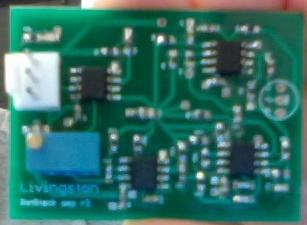
\includegraphics[width=2.5in]{figures/amp_r2_board.png}
\caption[Microphone amplifier board, r2]{A poor-quality photo of the
  current microphone amplifier board (``r2'', or ``release 2''). The
  power/signal cable attaches to the white 3-pin socket on the left
  and the microphone leads (not shown) attach near the right edge. The
  last high-gain stage is adjusted with the blue potentiometer on the
  bottom-left of the photo.}
\label{ampbrd2:fig}
\end{figure}

\begin{figure}
\centering
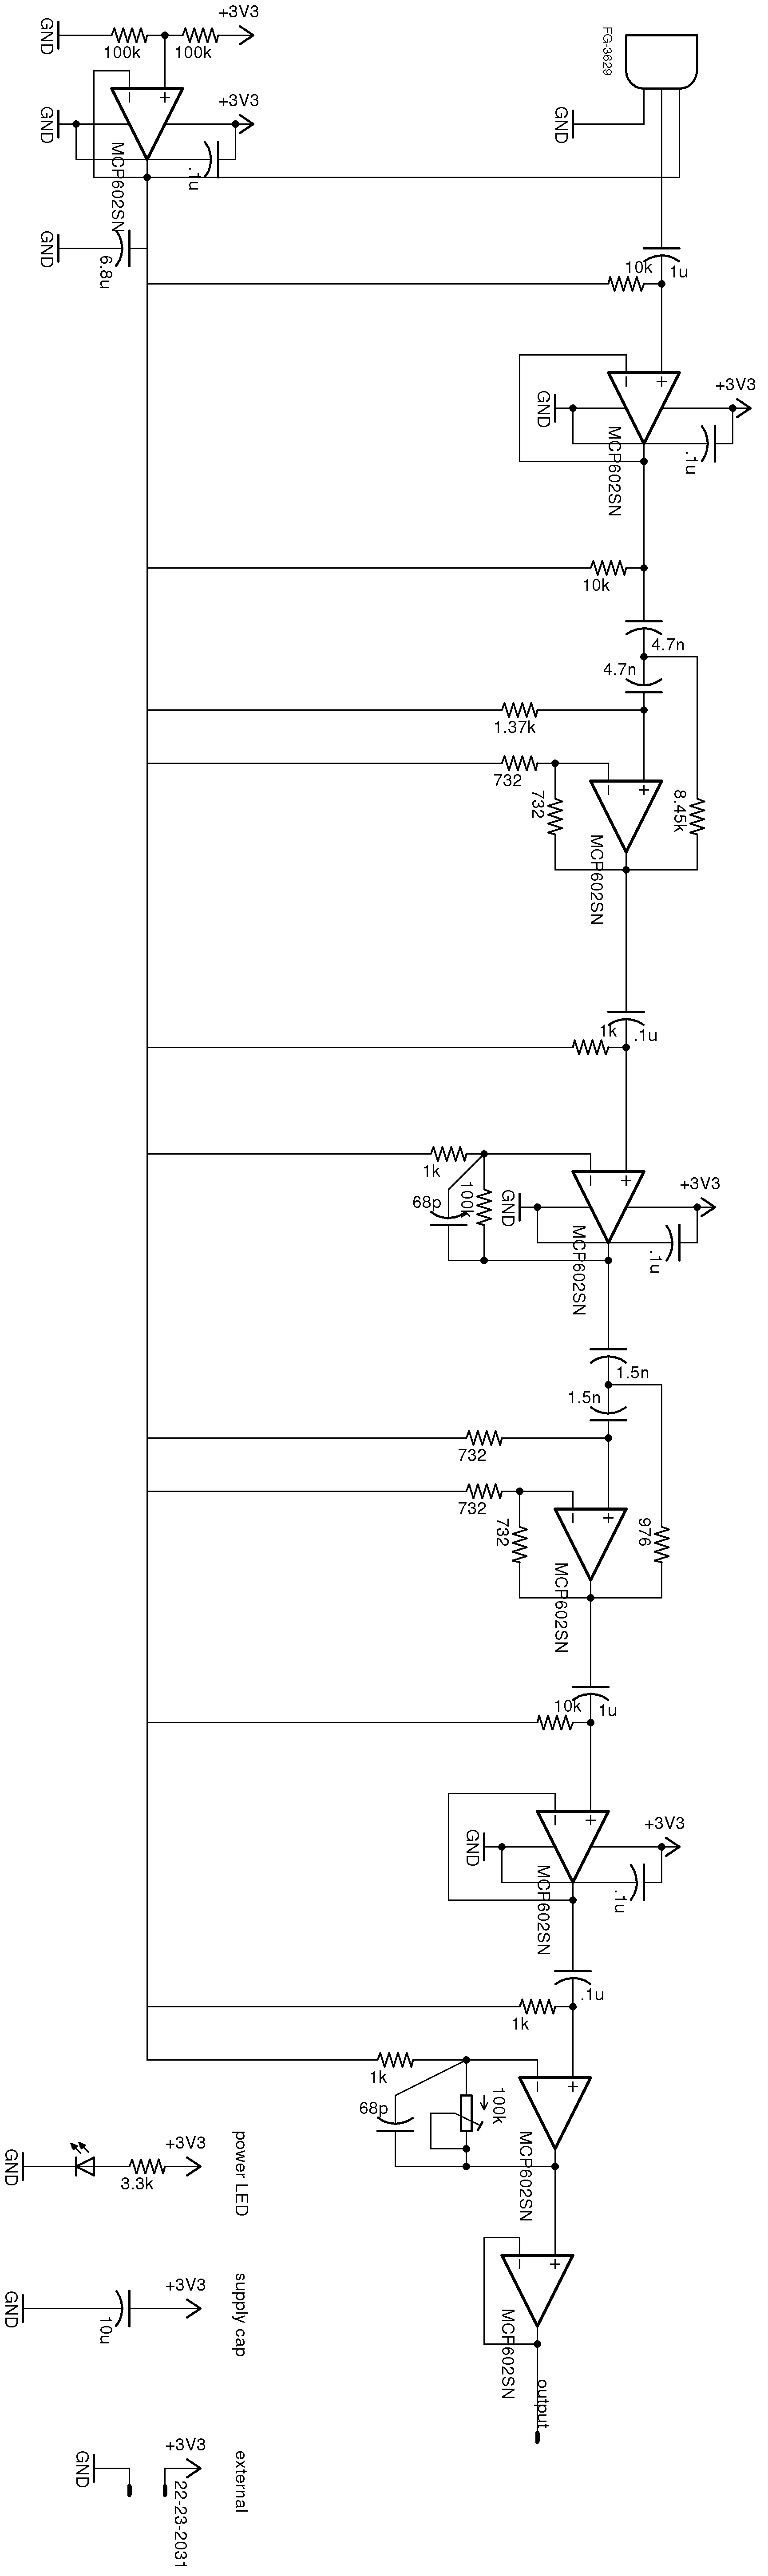
\includegraphics[height=\textheight]{figures/mic_amp_schematic.png}
\caption{Circuit schematic of microphone amplifier.}
\label{micamp_schem:fig}
\end{figure}

\subsection{MCU and memory boards}
\label{mcumemhardware:sec}

Circuit schematic in Fig.~\ref{mcubrd_schem:fig}.

The MCU is surrounded by various communication headers. These are
\begin{itemize}
\item ICSP\footnote{In-Circuit System Programming.} --
  Table~\ref{icsp_hdr:tbl},
\end{itemize}

\begin{table}[h]
\caption{Standard ICSP header}
\label{icsp_hdr:tbl}
\centering
\begin{tabular}{|l|c|}
\hline
\textbf{Label}&\textbf{Pin}\\
\hline
\hline
!MCLR & 1\\
\hline
Vdd & 2\\
\hline
GND & 3\\
\hline
PGD & 4\\
\hline
PGC & 5\\
\hline
\end{tabular}
\end{table}

\begin{figure}
\centering
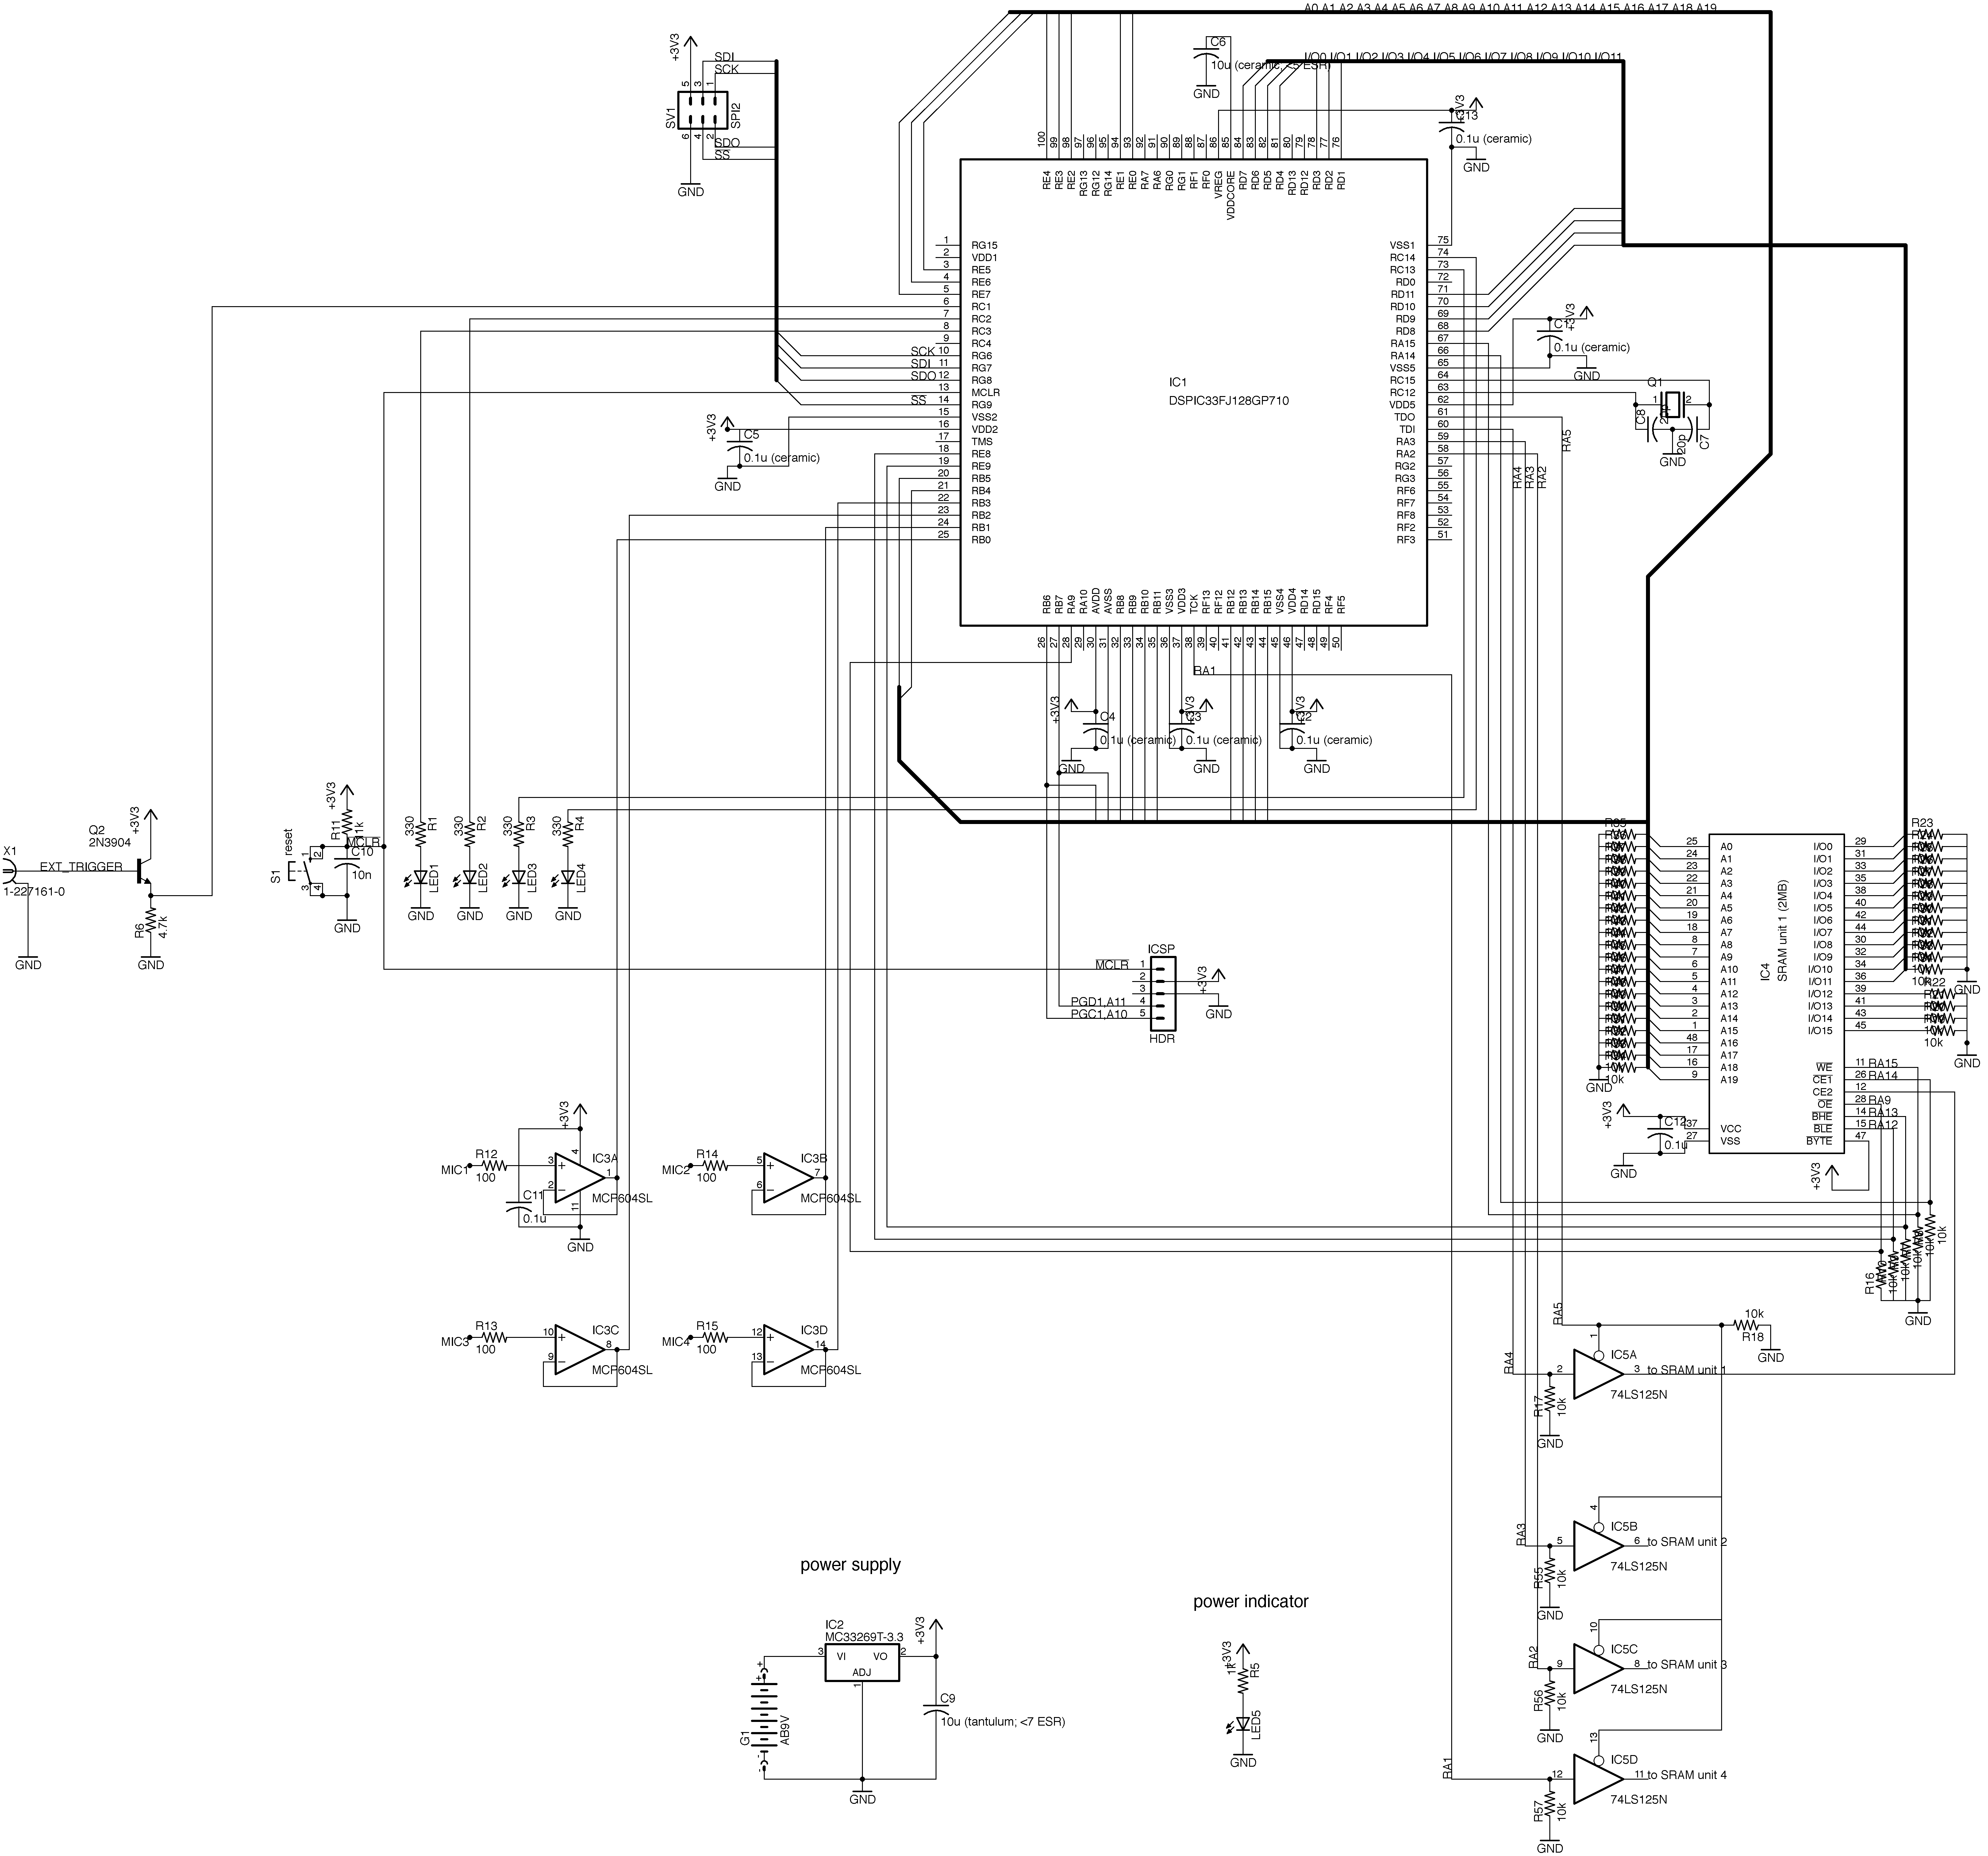
\includegraphics[width=\textwidth]{figures/mcu_board_schematic.png}
\caption[Circuit schematic of microcontroller and memory
  boards]{Circuit schematic of MCU and memory boards. Note that
  \textit{only one SRAM module is shown.} The SRAM chips have a common
  address bus and data bus, though the figure does not clearly show
  this.}
\label{mcubrd_schem:fig}
\end{figure}

\subsection{Other}

The schematic for the gain calibration tool is in
Fig.~\ref{gaincal_schem:fig}. Notice the trigger output is near the
left-side. It is a simple arrangement where the output is pulled to
ground (through the 4.7~k$\Omega$ resistor) while the NPN transistor
is ``off'', and brought quickly to 3.3~V (or ``high'') as a trigger
signal when the microcontroller switches the NPN transistor ``on.''

\begin{figure}
\centering
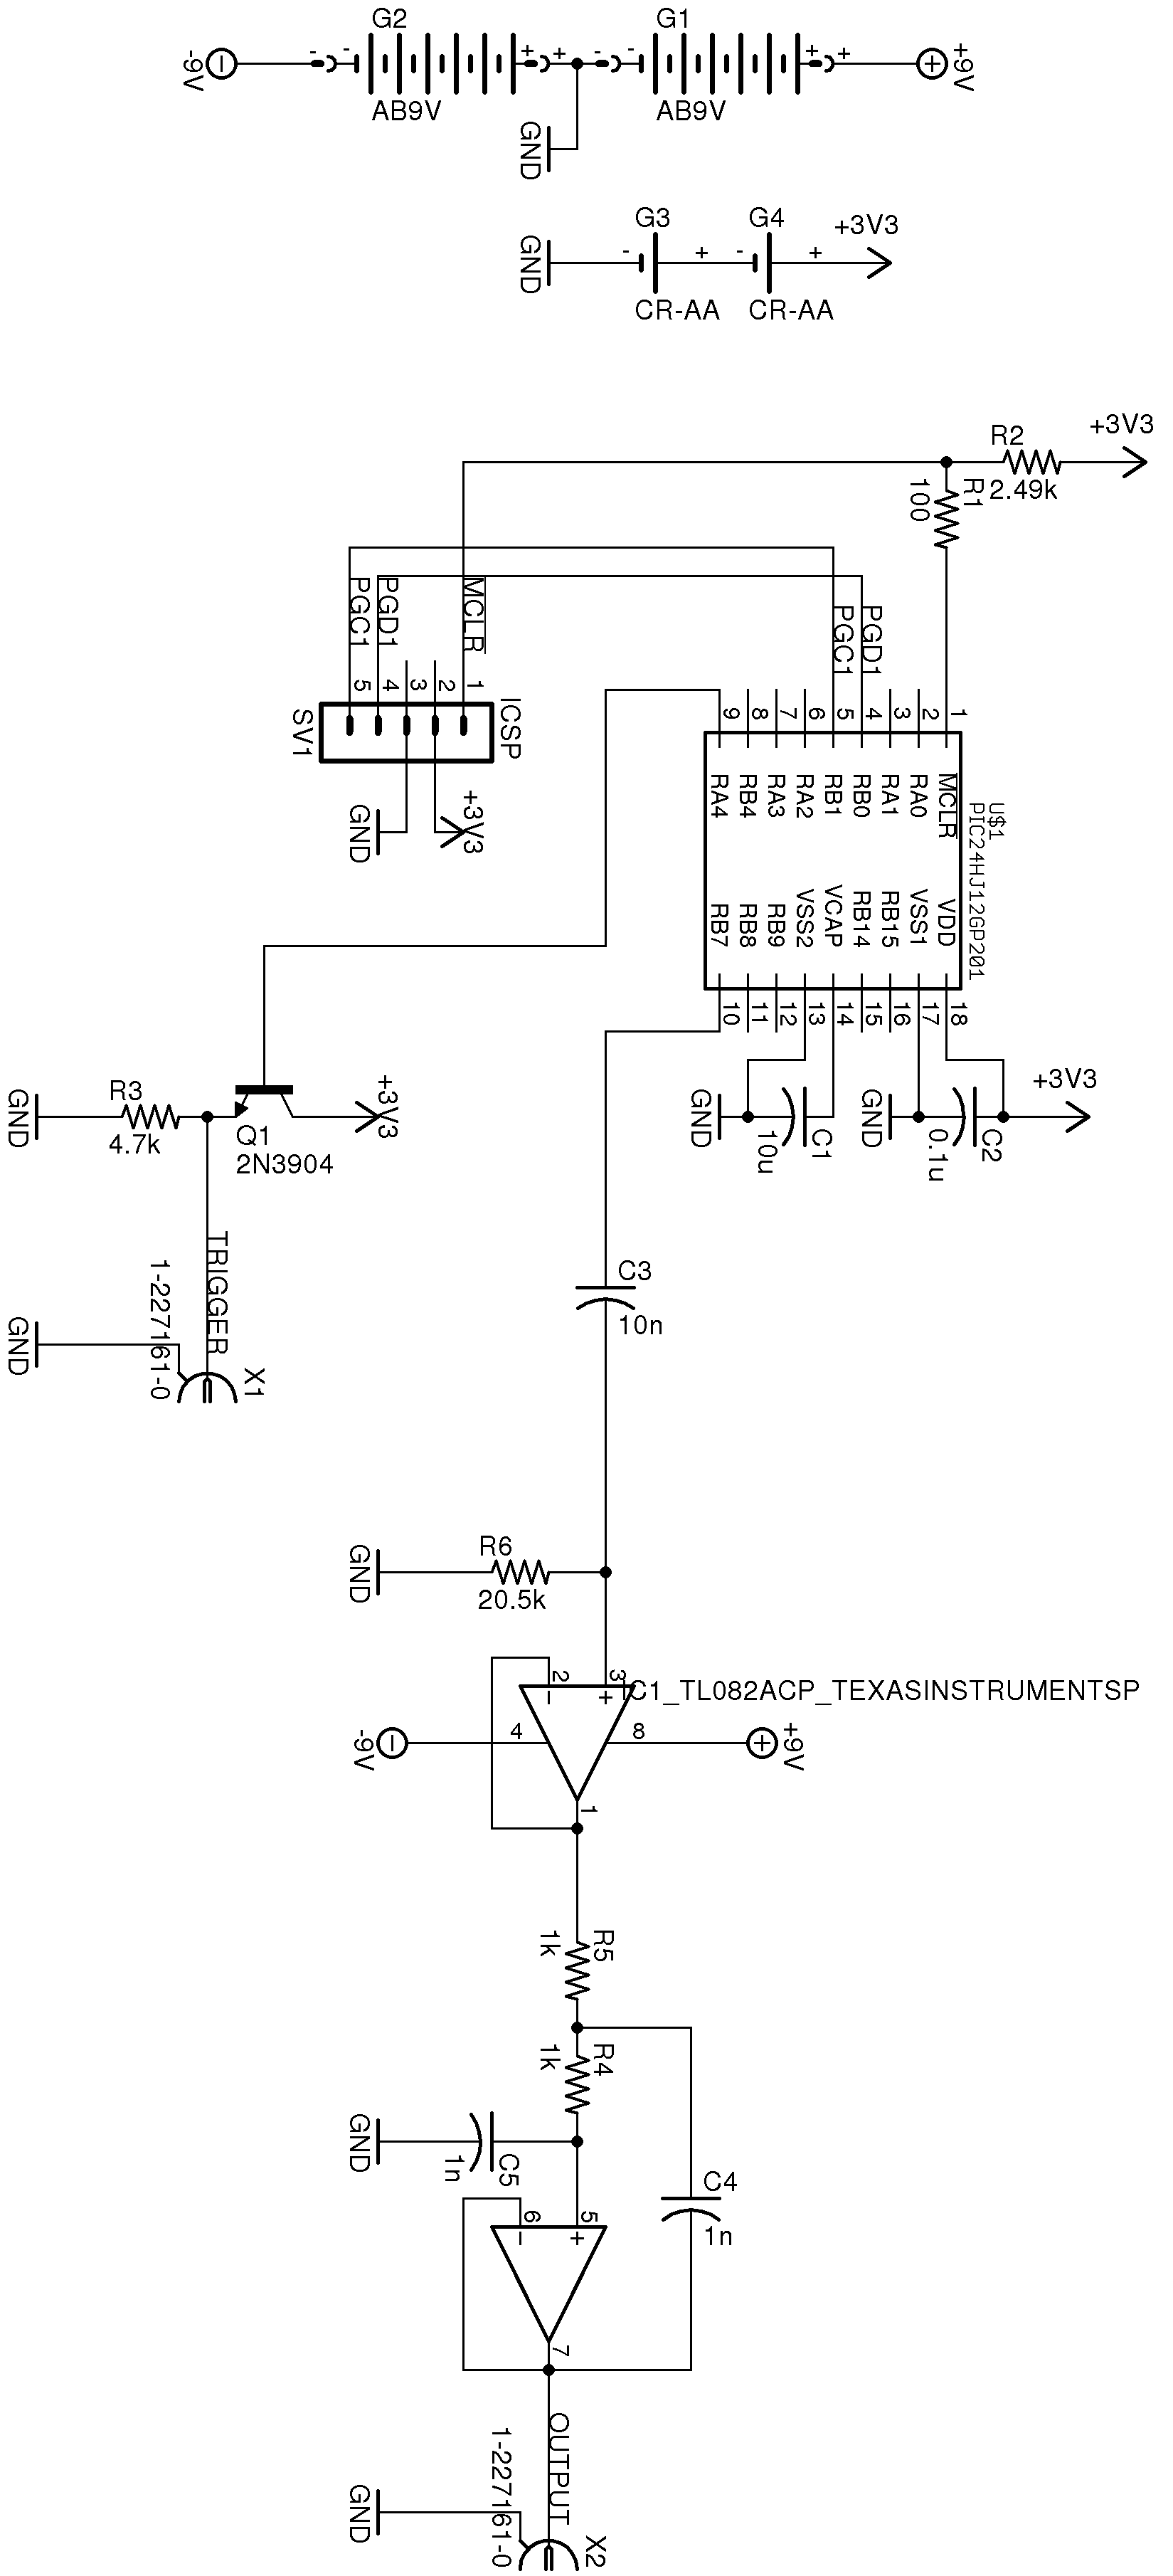
\includegraphics[height=\textheight]{figures/gaincal_schematic.png}
\caption[Gain calibration circuit]{Gain calibration circuit. The odd
  X1 and X2 semi-circular symbols are supposed to indicate a
  BNC/coaxial cable socket, where cable shielding connects to ground.}
\label{gaincal_schem:fig}
\end{figure}


\subsection{Bill of materials} % What to purchase, and where (recommended)

See Tables \ref{mic_parts:tbl} and \ref{mcu_parts:tbl}.  As mentioned
above, some of these part values are flexible. E.g., the 6.8 $\mu$F
decoupling capacitor could be increased in value. Do not be afraid to
try variations because these passive components are typically quite
cheap and can easily/safely be changed with a decent soldering
station. Generally you should buy components with tight tolerance
values, e.g. $1\%$ or better, in order to improve filter quality (or at
least, repeatability).

The 3-pin header on microphone amplifier boards is best mated with
Molex 3-pin 0.1'' house (part number 22-01-3037).

I have bought most often from Digikey (\url{http://www.digikey.com/})
but have also had good times with Mouser
(\url{http://www.mouser.com/}). In any case, Octopart
(\url{http://octopart.com/}) is an excellent way to find datasheets,
and parts availability at (potentially obscure) suppliers.

\begin{table}[h]
\caption{Microphone amplifier parts}
\label{mic_parts:tbl}
\centering
\begin{tabular}{|l|l|c|r|}
\hline
\textbf{Name}&\textbf{Package}&\textbf{Count}&\textbf{P/N}\\
\hline
\hline
Knowles FG-3629 & \textit{n/a} & 1 & ...\\
\hline
MCP6022 & 8-SOIC & 4 & MCP6022-I/SN\\
\hline
Molex 3 pin 0.1'' header & \textit{n/a} & 1 & 22-23-2031\\
\hline
0.1 $\mu$F (ceramic) & 0603 & 6 & ...\\
\hline
1.5 nF (ceramic) & 0603 & 2 & ...\\
\hline
1 $\mu$F (ceramic) & 0603 & 2 & ...\\
\hline
3.3 k$\Omega$ & 0603 & 1 & ...\\
\hline
4.7 nF (ceramic) & 0603 & 2 & ...\\
\hline
6.8 $\mu$F (ceramic) & 0805 & 1 & ...\\
\hline
8.45 k$\Omega$ & 0603 & 1 & ...\\
\hline
10 $\mu$F (ceramic) & 0805 & 1 & ...\\
\hline
68 pF (ceramic) & 0603 & 2 & ...\\
\hline
732 $\Omega$ & 0603 & 5 & ...\\
\hline
976 $\Omega$ & 0603 & 1 & ...\\
\hline
100 k$\Omega$ (pot) & triangle (5$\times$2.5 mm) & 1 & PV36Y104C01B00\\
\hline
100 k$\Omega$ & 0603 & 3 & ...\\
\hline
10 k$\Omega$ & 0603 & 3 & ...\\
\hline
1 k$\Omega$ & 0603 & 4 & ...\\
\hline
1.37 k$\Omega$ & 0603 & 1 & ...\\
\hline
LED (green) & 0603 & 1 & ...\\
\hline
\end{tabular}
\end{table}

\begin{table}[h]
\caption{MCU and memory boards parts}
\label{mcu_parts:tbl}
\centering
\begin{tabular}{|l|l|c|r|}
\hline
\textbf{Name}&\textbf{Package}&\textbf{Count}&\textbf{P/N}\\
\hline
\hline
3.3V regulator (800~mA) & DPAK & 1 & MC33269DT-3.3GOS-ND\\
\hline
74LVT125DB (quad buffer; 3-state) & 14-SSOP & 1 & \ldots\\
\hline
16~Mbit Static RAM & 48-TSOP & 4 & CY62167DV30LL-55ZXI\\
\hline
NPN BJT (discrete; 200~mA) & TO-92 & 1 & 2N3904BU\\
\hline
\end{tabular}
\end{table}

\subsection{Notes on old editions}

ExpressPCB\footnote{\url{http://expresspcb.com/}} was previously the
preferred boardhouse, largely because they offer such competitive
prices and fast delivery for small/specialty-run prototypes. In the
BatStack sourcetree, under the directory \texttt{hardware/archived},
we have
\begin{description}
\item[DsPICBoardMicrophoneConnector.pcb] microphone amplifier cable header
  board (4 headers total) -- created largely as a patch to earlier MCU
  board designs;
\item[micamp.pcb] microphone amplifier -- should be indexed as ``v1.5'';
\item[Prototype\_ADC\_SDCARD\_IC\_Test\_Board\_v3.3.pcb] MCU board;
\item[SRAM\_Prototype\_1.3.pcb] memory (or ``SRAM'') board;
\item[custom\_expresspcb] directory of custom symbols and footprints
  for ExpressPCB layout and schematic drawing software.
\end{description}

\subsubsection{MCU board}
\label{oldmcu:sec}

Older editions use the LV 24-33 MCUCard for dsPIC33FJ128GP710
(100-TQFP\footnote{100 pins, thin quad-flat package.} footprint), as
released by Mikroelectronika, Inc.

The ICSP port on older boards is in a non-standard configuration. From
left to right, the pins are
\begin{enumerate}
\item Vdd -- power suppy, 3.3V,

\item PGD -- programmer data line,

\item PGC -- programmer clock line,

\item $\overline{\textrm{MCLR}}$ -- MCU reset (or ``clear'').

\item GND -- ground.
\end{enumerate}

The SD card SPI interface header --5$\times$2 male header, 0.1"
spacing-- on the left side of the board (in Fig.~\ref{oldmcu:fig}) has
pin labels as in Table~\ref{old_sdspi_hdr:tbl}, again with the typical
orientation, as in Fig.~\ref{oldmcu:fig}. We use the notation SDI and
SDO for dsPIC33F chip SPI module input and output, respectively, as in
the device datasheet\footnote{dsPIC33FJXXXGPX06/X08/X10 Data Sheet,
  \url{http://ww1.microchip.com/downloads/en/DeviceDoc/70286C.pdf}}. Deciding
which corresponds to ``MISO'' and which to ``MOSI'' (i.e., standard
SPI terminology), depends on your particular configuration, that is
whether the dsPIC33F is acting as master or slave. For SD card
communication, the SD card controller is the slave.

\begin{table}[h]
\caption{SD/SPI header labels, old MCU board}
\label{old_sdspi_hdr:tbl}
\centering
\begin{tabular}{|l|c|c|r|}
\hline
\textbf{Label}&\textbf{Pin}&\textbf{Pin}&\textbf{Label}\\
\hline
\hline
GND & 1 & 2 & Vdd (3.3~V)\\
\hline
 & 3 & 4 & \\
\hline
SDO (MOSI) & 5 & 6 & SDI (MISO)\\
\hline
SCK & 7 & 8 & SS\\
\hline
 & 9 & 10 & \\
\hline
\end{tabular}
\end{table}

In Appendix~\ref{oldsnapshots:sec}, images of the old layout for MCU
and memory boards are in Fig.~\ref{oldmcu_layout:fig} and
Fig.~\ref{oldmem_layout:fig}, respectively.

A populated exemplar MCU board is shown in Fig.~\ref{oldmcu:fig};
position references in the following are with respect to this
figure. It consists of
\begin{itemize}
\item \underline{external power jack} -- (black, large, in upper-left
  corner) attachment point for battery or other DC voltage
  supply. This connects directly to the voltage regulator (i.e. there
  is no fuse/shock protection; please be careful).

\item \underline{3.3V regulator} -- (upper-left of figure, next to
  external power jack) MC33269DT-3.3 , provides 3.3~V to the Stack;
  becomes quite hot (too hot?) during operation.

\item \underline{SD/SPI header} -- (left side of figure); 5$\times$2
  (0.1" spacing) header; provides SPI bus to SD card. Usual SPI pins
  are present: power (Vcc), ground (GND), SS\footnote{slave select.},
  SCK\footnote{clock; recall that SPI is a synchronous, full-duplex
    protocol.}, MOSI\footnote{master-out, slave-in.},
  MISO\footnote{master-in, slave-out.}. Thus, 4 of the 10 header pins
  are unused. Note that power (Vcc) is the same supply as for the rest
  of the Stack: 3.3~V, from the regulator.

\item \underline{Reset button} -- (lower left corner of Figure) drops
  \mbox{!MCLR} pin low, causing the dsPIC33F chip to
  reset\footnote{formally called a ``Master Clear Pin Reset'', but
    essentially leads to the same result as other reset methods.}. For
  the firmware in use at the time of writing, you should use this
  button to restart a Stack when some non-fatal error is made (by you,
  a user of the Array), thus returning (hopefully) to the
  ready-for-trigger state.

\item \underline{trigger pin} -- (lower left corner of Figure, next to
  Reset button; in particular, the left of the two pins) connects to a
  pin on the dsPIC33F chip that is used for triggering a
  recording. Note that \textit{this lacks a needed buffer for
    receiving an external TTL pulse}. See left side of
  Fig.~\ref{mcubrd_schem:fig} for the solution\footnote{basically, NPN
    BJT with 4.7~k$\Omega$ resistor between ground and emitter,
    collector connected to Vcc, external input at base, and output (to
    trigger pin on MCU board) from emitter.}. Also see notes in
  Sec.~\ref{triggering:sec}.

\item \underline{green indicator LEDs} -- (4 total) provide a limited
  reporting mechanism for the firmware. Indeed, 16 ($= 2^4$) messages
  are possible, unless we incorporate sequential encoding; see
  Sec.~\ref{errorcode:sec} for current error codes.

\item \underline{outdated microphones header} -- (along bottom edge of
  Figure, mid-left) once upon a time, acted as header for ribbon cable
  that provided power and signal for separate microphone boards,
  configured in a stack of PCBs. A small adaptor board provides the
  current 3-pin amplifier cable header for four channels, and connects
  to this much older 5$\times$2.

\item \underline{input (unity) buffer} -- (near middle of board, just
  to left of dsPIC33F socket) buffers input from microphone amplifier
  boards to ADC pins on microcontroller; uses MCP6024 quad op amp
  chip, all in unity gain configuration. Note that each channel input
  is led by a series 1~k$\Omega$ resistor for, among other
  possibilities, safety. This could (should?) be replaced by something
  smaller, e.g. 100~$\Omega$.

\item \underline{dsPIC33F breakout socket} -- (four large, black 2-row
  female connection boxes; arranged in a square; compare with
  Fig.~\ref{mikropic:fig}) attachment point for dsPIC33FJ128GP710
  breakout board, as released by Mikroelektronika company. Decoupling
  and tank capacitors, and a clock crystal are on this board (hence,
  not included in the original MCU board).

\item \underline{memory board socket} -- (only solder points are
  visible in the Figure; compare with Fig.~\ref{oldmem:fig}) houses
  address, data and control lines between MCU and SRAM chips.

\item \underline{ICSP header} -- (bottom right, next to I2C header)
  programming interface; non-standard pin order, as noted above. Next
  to the header are two jumpers (red-insulated wires in the
  Figure). These are for the clock and data lines (PGC and PGD, resp.)
  and can be left always connected (as they are in the Figure).

\item \underline{I2C header} -- (bottom right corner; lacks header
  pins in Figure) direct connect to I2C pins on dsPIC33F chip. Only 4
  pins are required (as standard with I2C): power, ground, SDA and
  SCL. Unused at time of writing. Note that pull-up resistors must be
  added externally to use an I2C bus here.
\end{itemize}


\section{Firmware}
\label{firmware:sec}

[COMMENTS ABOUT IDIOSYNCRACIES WITH PIC C30 HEX CODING.]

\subsection{Organization}

Note that the SD card SPI interface code controls the slave select
(SS; also called ``chip select'' or ``CS'') pin manually because there
is a bug in the dsPIC33F SPI module hardware\footnote{still a problem
  as of silicon revision A4; see errata sheet at
  \url{http://ww1.microchip.com/downloads/en/DeviceDoc/80446D.pdf}}.

\begin{description}
\item[\texttt{batstack\_id}] 8-bit address (or ``ID'') of the
  BatStack. Reserved values are
  \begin{description}
  \item[\texttt{0x00}] uninitialized SD card (or storage medium for
    trial data, more generally);
  \item[\texttt{0xFF}] broadcast address.
  \end{description}

\item[\texttt{posttrigger\_len}] number of blocks to record
  \textit{after} trigger.

\item[\texttt{build\_date}] 16-bit encoded date on which firmware was
  built; this is \textit{not} automatically set, and serves primarily
  as a simplified versioning method. See Sec.~\ref{bulkmemorg:sec} for
  specification.
\end{description}

\subsection{Memory organization on SD card}
\label{bulkmemorg:sec}

Because SD cards are block devices, where a block (or ``sector'') is
512 bytes long, large and logically separate units of data on the SD
card are aligned to blocks. Note however that this basic organization
of trial data on the SD card could be applied to other forms of memory
storage.

Grossly speaking, the trial data is stored consecutively in
chronological order following the header, and the header provides
information about the installed firmware and various settings and
stores a list of links and timestamps for trials. Specifically, the
first two sectors of memory, i.e. the first 1024 bytes, serve as the
header, which is organized as follows by byte addresses:
\begin{itemize}
\item[0] BatStack ID -- see previous section for reserved addresses;
\item[1-2] firmware build date (or \texttt{BDATE}), where
  \texttt{BDATE}$<$4:0$>$ is day, \texttt{BDATE}$<$8:5$>$ is month,
  and \texttt{BDATE}$<$15:9$>$ is year (in years since 1970, i.e. add
  1970 to this value);
\item[3] \textit{high nibble} is (unsigned) sample width (should be 0xA), and
  \textit{low nibble} is microphone ``active'' flags, 1 bit per channel, value
  of 1 indicating channel in use;
\item[4-5] sample period in 10 ns units;
\item[6-7] post-trigger length (or \texttt{POSTLEN}), i.e. number of
  256-sample (per channel) blocks to be recorded after the trigger;
\item[8] (unsigned) number of trials recorded;
\item[9-] trial data links, where each entry is 12 bytes wides and provides
  \begin{itemize}
  \item[0-3] sector address (marks start of trial recording) -- this must be multiplied by 512 to get the byte address;
  \item[4-5] date (same format as \texttt{BDATE});
  \item[6-7] time of day in decaseconds (i.e. tens of seconds) since
    midnight -- combining with previous date field gives a complete
    timestamp;
  \item[8-9] \texttt{POSTLEN} at time of this trial recording;
  \item[10-11] \textit{reserved}, \ldots likely will hold sample period at time of recording\ldots
  \end{itemize}
\end{itemize}
Note that all multi-byte fields have little endian ordering.

The BatStack firmware uses the sample period field as an indicator of
whether recording parameters should be read (and used) from the SD
card or set to default (i.e. compiled) values. Specifically, if sample
period is 0 per header, then assume header parameters are unset. This
will often be the case for virgin SD cards (not yet paired with a
Stack).


\subsection{Error codes}
\label{errorcode:sec}

If an error occurs on a BatStack that cannot be recovered from (so
called ``fatal errors''), then a four bit error code is printed on the
on-board LEDs and the machine halts. The orientation to read the
nibble is LSb to right if the board is viewed with trigger and reset
buttons in the upper right corner.
\begin{itemize}
  \item[\texttt{0001}] Oscillator error (trap);
  \item[\texttt{0010}] Address error (trap);
  \item[\texttt{0011}] DMAC\footnote{Direct Memory Access Controller.}
    write conflict (trap);
  \item[\texttt{0100}] SD card communication error (not necessarily
    fatal, but easier in this early implementation to be so);
  \item[\texttt{0101}] Math error (trap);
  \item[\texttt{0110}] Stack error (trap);
  \item[\texttt{1111}] Unhandled interrupt.
\end{itemize}


\subsection{Creating a build environment}
\label{createbuildenv:sec}

Before we begin, note that Microchip distributes a free (as in price,
not freedom) ``academic edition'' IDE\footnote{integrated development
  environment.} for PIC24H/dsPIC33F microcontroller families. This,
combined with one of their commerical programmers or the GoodFET
(\url{http://goodfet.sourceforge.net/}) under Windows, should suffice
to setup a build environment on a Windows box \textit{for developing
  firmware}. At the time of writing, the other tools
(e.g. \texttt{dumpsd}) expect a standard Unix (or GNU/Linux)
environment. Porting to Windows may prove difficult, unless --and this
is what I prefer-- the various tools are rewritten in Python.

We assume you are working on a modern GNU/Linux
system\footnote{Somewhere near Linux 2.6.32, GNU C Library 2.11.1 and
  GCC 4.4.3}. An additional key item, which you may not have
installed\footnote{not having this installed is good cause to feel
  embarrassed. Shame on you.}, is Python. Instructions for a standard
installation are on the \mbox{python.org} website:
\url{http://python.org/download/}. If you are using Debian or Ubuntu,
installation should be as simple as
\begin{verbatim}
# apt-get install python
\end{verbatim}
At the time of writing, the only
tool written in Python is \texttt{gendate.py}, which converts a given
date (i.e. year, month, day) to its 16-bit word representation
(cf. Sec. \ref{bulkmemorg:sec}).

The toolchain is an extension of GCC\footnote{GNU Compiler Collection,
  or GNU C Compiler.}, targeting the 16-bit PIC families released by
Microchip\footnote{these families are dsPIC33F, PIC24H, dsPIC30F, and
  PIC24F.}, and a non-free (as in, proprietary, i.e., not open source)
C library to link against. This non-free stuff is not needed if you
write in pure assembly. We must thus first build the compiler (and
assembler, linker, etc.), install it, copy in the non-free C library,
and then perform any post-installation configuration (e.g., mostly
setting path variables appropriately).

A Web author, whom I only know by the handle ``Matt'', wrote a good
tutorial on the setup process.
\url{http://www.electricrock.co.nz/blog/2009/08/installing-microchips-c-compiler-for-pic24-mcus-and-dspic-dscs-c30-on-ubuntu-9-04/}
I defer filling in details for the moment because I will need to
create a fresh toolchain soon myself, and will make any additional
notes at that time. For now, consider that
\begin{itemize}
\item I have successfully applied the above process to build and
  install Microchip's C30 v3.23b, beginning with a current and
  (mostly) typical Ubuntu distribution.

\item \textit{Do not} follow Matt's more recent article, ``Microchop
  C30 Compiler for Linux.'' The automated build script can fail in the
  middle of the build/installation process (as it did for me), and
  leave you with an incomplete result that is a bit tricky to undo (as
  it was for me). At most, I suggest you see what the build script
  does and perform each step manually, if appropriate.
\end{itemize}

\subsubsection{External resources}
\begin{description}
\item[GoodFET JTAG adaptor] \url{http://goodfet.sourceforge.net/}

\item[dsPIC33FJ128GP710]
  \url{http://www.microchip.com/wwwproducts/Devices.aspx?dDocName=en024676}

\item[16-bit PIC programmer's reference]
  \url{http://ww1.microchip.com/downloads/en/DeviceDoc/70157D.pdf} (If
  this link is dead, then look under documentation for the dsPIC33F
  chip above.)

\item[16-bit PIC assembler, linker]
  \url{http://ww1.microchip.com/downloads/en/DeviceDoc/DS-51317H.pdf}
  (If this link is dead, search for ``C30'' related downloads on
  Microchip's website; and notify Scott!)

\item[16-bit PIC C compiler]
  \url{http://ww1.microchip.com/downloads/en/DeviceDoc/51284J.pdf}
\end{description}


\section{Tools miscellany}
\label{misctools:sec}

This section is scatter-brained by construction. Have fun. And note
that not every little thing is mentioned here, and often times
comments written at the top (or in the midst) of source code files are
a better reference.

As with most software or firmware in the project, you can usually
assume that building is achieved by running \texttt{make} in the
appropriate directory. E.g., to build the imaginary \texttt{foobar},
\begin{verbatim}
$ cd /some/random/path/to/BatStack
$ cd src/foobar
$ make
\end{verbatim}
This requires a Makefile. Look in any of these Makefiles for details
of the orchestrated build process\footnote{Do not worry; the build
  scripts are not auto-generated. I wrote them by hand.}.

If you do not see the program that interests you mentioned below, then
try looking toward the top of the source code file for
documentation. For Octave/Matlab scripts, 
\begin{verbatim}
>> help spicegirl
\end{verbatim}
might return helpful information about using the \texttt{spicegirl}
function. If you are still lost, then please contact me, Scott
Livingston. Email is preferred.

Here is a laundry list. Paths are relative to the BatStack sourcetree
root. For some programs, passing ``-h'' as an argument causes usage
notes to be printed (e.g., \texttt{gendate.py}). For others, calling
the program with no arguments --when some are mandatory-- will cause a
usage message to be printed (e.g., \texttt{dumpsd}).
\begin{description}
\item[util/\texttt{batstack}] (a Python module); Please see help
  documentation within the module for usage, details, etc.  From the
  command-line, try something like
\begin{verbatim}
$ cd src/util
$ pydoc batstack
\end{verbatim}
where I included ``cd src/util'' to remind you to change to the
directory where \texttt{batstack.py}; of course, this is not necessary
if the directory is in your \texttt{PYTHONPATH}. For newbies, note
that we do not include the trailing ``*.py'' when using \texttt{pydoc}
(the Python documentation tool), i.e. the actual file is
\texttt{src/util/batstack.py}.

\item[util/\texttt{memcheck}] Check an attached memory board to verify
  that read and write operations work correctly. The approach used is
  not complete, and for the code revision at time of writing, some
  types of errors can slip by undetected during this check.

\item[util/\texttt{gendate.py}] Encode the given date in the 16-bit
  container used by the firmware
  (cf. Sec.~\ref{bulkmemorg:sec}). Running without arguments will use
  today as the date (as reported by the host operating system). E.g.,
  if I run it now on my laptop, (copy-and-pasted from my terminal)
\begin{verbatim}
$ ./gendate.py
Using today (i.e. 26/09/2010)
0x513A
\end{verbatim}
  To specify a specific date, use the form ``YYYY MM DD''. E.g., for
  February 12, 2009, (again, copy-and-pasted)
\begin{verbatim}
$ ./gendate.py 2009 2 12
0x4E4C
\end{verbatim}

\item[util/legacy/\texttt{update12.py}] Convert Array data files
  (cf. Sec.~\ref{array_format:sec}) from file
  spec\footnote{\textit{Jargon:} ``spec'' abbreviates
    ``specification.'' More generally it can refer to a formal
    standard or format.} version~1 to version~2.
\end{description}

\section{Tips \& tricks, or ``saving the youth''}
\label{tips:sec}

Here we list various unsorted but important notes on building, using,
debugging, etc. the Batlab Microphone Array. Hopefully these tips are
non-obvious and will save you from many hours of suffering.

\begin{itemize}
\item We are interested in an acoustic signal of brief duration and
  large dynamic range. 

\item While we are still using SD cards for bulk local memory storage,
  I \textit{highly} advise using Sandisk brand 2 GB cards. Other sizes
  should (and have) worked fine, but 2 GB SD cards have been tested
  the most. I have tried a different brand of SD card (the name of
  which I cannot recall\ldots{} it is white-ish and sold in the UMD
  STAMP Student Union bookstore), and it was horidly buggy and slow. A
  possible reason for this is that some vendors deviate from the
  published SD over SPI protocol, which is precisely what I used while
  writing read/write routines for such memory. This explanation is
  justified even if decent performance is obtained when such a SD card
  is used in a desktop computer because many operating system device
  drivers are designed to handle deviations from published standards,
  and possibly, the SD native communication mode may be properly
  implemented while only half-assed SPI support is provided.

\item Pay attention to triggering. Notice the
\begin{itemize}
\item network of connections with the trigger source,
\item (nominal) electrical characteristics of the trigger source,
\item what sort of ``load'' the receiving (i.e. ``triggered'') devices
  represent, and
\item timing of the final system!
\end{itemize}
There should be some notes in this regard on the Batlab Wiki website,
``wikibat.'' The basic tips are to ensure all devices on the trigger
line are powered on (and waiting for an external trigger) and that
none of them will do something unneighborly to the shared line after
being triggered, e.g. pulling it low and possibly preventing other
devices from ever getting triggered.

\item If you are developing the firmware, then be aware that the C30
  compiler (a port of gcc; also variously called ``PIC30'' or
  ``pic30-coff'') can generate flawed assembly, which can lead to
  subtle stack alignment errors that later cause traps. The debugging
  lesson: in addition to the C code, do not be afraid to consider the
  assembly code. \texttt{objdump} is your friend.

\end{itemize}


\appendix

\section{Snapshots of old layout}
\label{oldsnapshots:sec}

Figs.~\ref{oldmcu_layout:fig}--\ref{oldmem_layout:fig}; these are
screenshots of ExpressPCB layout. Red is top layer, green is bottom
layer, yellow is silkscreen. Note that since we bought ``prototype''
boards, there was no silkscreen (nor soldermask, etc.).

\textbf{N.B.}, the MCU board layout in Fig.~\ref{oldmcu_layout:fig}
does not perfectly match the boards you have on hand. Indeed,
\textit{you should not have this fabricated} because it includes at
least one error, and even an unused (i.e. ``floating'' or
``unconnected'') 2$\times$5 socket in the lower left.

\begin{figure}
\centering
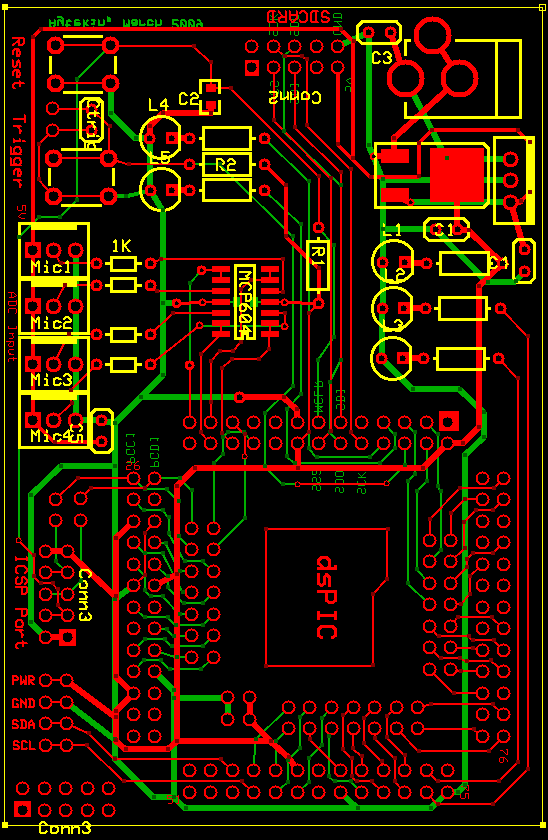
\includegraphics[height=\textheight]{figures/old_mcu_layout.png}
\caption[Old microcontroller board layout using ExpressPCB]{Old MCU
  board layout using ExpressPCB software.}
\label{oldmcu_layout:fig}
\end{figure}

\begin{figure}
\centering
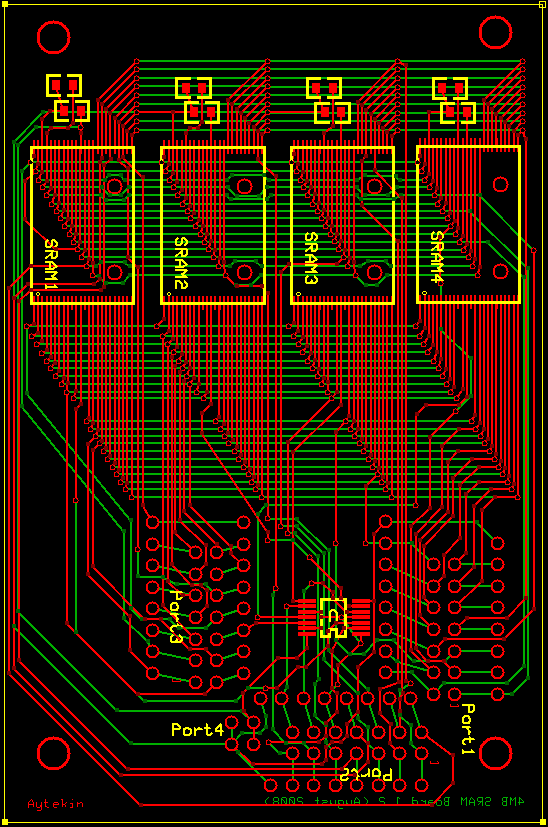
\includegraphics[height=\textheight]{figures/old_mem_layout.png}
\caption[Old memory board layout using ExpressPCB]{Old memory (or
  ``SRAM'') board layout using ExpressPCB software.}
\label{oldmem_layout:fig}
\end{figure}

\section{Additional resources}
% Links to websites, book references, etc. that would be helpful in
% constructing and understanding the mic array.
\begin{itemize}
\item \url{http://octopart.com/} for datasheets, and parts
  availability at many suppliers (aside from Digi-Key and Mouser).

\item \url{http://wiki.hacdc.org/index.php/Suppliers} for an excellent
  directory (at time of writing) of electronics stores, boardhouses,
  CNC/millhouses, materials suppliers, etc. This website is organized
  by DC's hackerspace, HacDC. Their website is
  \url{http://www.hacdc.org/}.
\end{itemize}

\section*{Acknowledgments}

Murat Aytekin, who began the project.  Lakshmi Krishnan for
photographs of array hardware.  Ben Falk and Mel Wohlgemuth for great
discussions.  Others who will be thanked when this is not a
draft\ldots Special thanks is sent out to all the bats of my life.


\end{document}
